\documentclass[12pt,a4paper]{article}
\usepackage[utf8]{inputenc}
\usepackage[T1]{fontenc}
\usepackage{amsmath,amsfonts,amssymb}
\usepackage{geometry}
\usepackage{graphicx}
\usepackage{booktabs}
\usepackage{float}
\usepackage{hyperref}
\usepackage{natbib}

\geometry{margin=1in}

\begin{document}

\begin{titlepage}
\begin{center}

\vspace*{1.5in}

{\Large \textbf{STATISTICAL ANALYSIS OF INSURANCE CHARGES: \\
A PREDICTIVE MODELING STUDY}}

\vspace{1in}

{\large BY}

\vspace{0.2in}

{\large PABLO LEYVA}

\vspace{0.2in}

{\large pl33@njit.edu}

\vspace{1.2in}

{\large Project One Report}

\vspace{0.2in}

{\large Submitted in completion of the requirements \\
for the course of Statistical Learning Capstone}

\vspace{1in}

{\large New Jersey Institute of Technology}

\vspace{0.2in}

{\large Newark, New Jersey}

\vspace{0.3in}

\end{center}
\end{titlepage}

\begin{abstract}
This study presents a comprehensive statistical analysis of insurance charges using demographic and health-related predictors. We employed linear regression and Ridge regression techniques to identify key factors influencing insurance costs and develop predictive models. Our analysis reveals that smoking status is the most significant predictor of insurance charges, followed by the number of children, BMI, age, region, and sex. The final linear regression model achieved an R-squared value of 0.769, explaining approximately 77\% of the variance in insurance charges.
\end{abstract}

\section{Introduction to the Study}

Healthcare costs and insurance premiums have become increasingly important topics in modern society. Understanding the factors that influence insurance charges is crucial for both insurance companies in risk assessment and for individuals in making informed healthcare decisions. This study analyzes a comprehensive dataset of insurance charges to identify the key demographic and health-related factors that drive insurance costs.

\section{Objective}

The primary objectives of this study are:

\begin{enumerate}
    \item \textbf{Exploratory Analysis}: To conduct comprehensive exploratory data analysis to understand the distribution of insurance charges and identify patterns in the relationship between predictor variables and insurance costs.
    
    \item \textbf{Feature Assessment}: To evaluate the relative importance of demographic and health-related factors (age, sex, BMI, number of children, smoking status, and geographical region) in predicting insurance charges.
    
    \item \textbf{Predictive Modeling}: To develop and evaluate linear regression models for predicting insurance charges, including regularized models to handle potential overfitting.
    
    \item \textbf{Model Validation}: To assess model performance using appropriate statistical metrics and diagnostic tests to ensure model reliability and validity.
    
    \item \textbf{Policy Insights}: To provide actionable insights that can inform insurance pricing strategies and help individuals understand factors affecting their insurance premiums.
\end{enumerate}

These objectives aim to provide a comprehensive understanding of insurance charge determination and develop robust predictive models that can serve both academic and practical purposes in the insurance industry.

\section{Statistical Analysis}

\subsection{Data Description and Preprocessing}

The dataset comprises 1,338 observations with seven variables:
\begin{itemize}
    \item \textbf{Age}: Continuous variable (integer values)
    \item \textbf{Sex}: Binary categorical variable (male/female)
    \item \textbf{BMI}: Continuous variable representing body mass index
    \item \textbf{Children}: Discrete variable indicating number of dependents
    \item \textbf{Smoker}: Binary categorical variable (yes/no)
    \item \textbf{Region}: Categorical variable with four levels (southeast, southwest, northeast, northwest)
    \item \textbf{Charges}: Continuous dependent variable (insurance charges in USD)
\end{itemize}

Data preprocessing involved encoding categorical variables using appropriate techniques:
\begin{itemize}
    \item Sex and smoker status were encoded using dummy variables with drop\_first=True
    \item Region was mapped to numerical values (southeast=0, southwest=1, northeast=2, northwest=3)
    \item Data types were optimized for memory efficiency: age, children, and region variables were converted to \texttt{uint8}, while BMI and charges were converted to \texttt{float32}, resulting in a 25\% memory reduction (from 73.3+ KB to 55.0 KB)
\end{itemize}

\subsection{Exploratory Data Analysis}

The exploratory analysis revealed several key insights:

\subsubsection{Distribution Analysis}
Insurance charges exhibited a right-skewed distribution with mean charges significantly higher than median charges. The data appears to be normally distributed but right-skewed, as evidenced by the log transformation which reveals an underlying normal distribution. This suggests the presence of multiplicative effects in the data, where certain factors may compound to create extremely high charges for specific subgroups.

\begin{figure}[H]
\centering
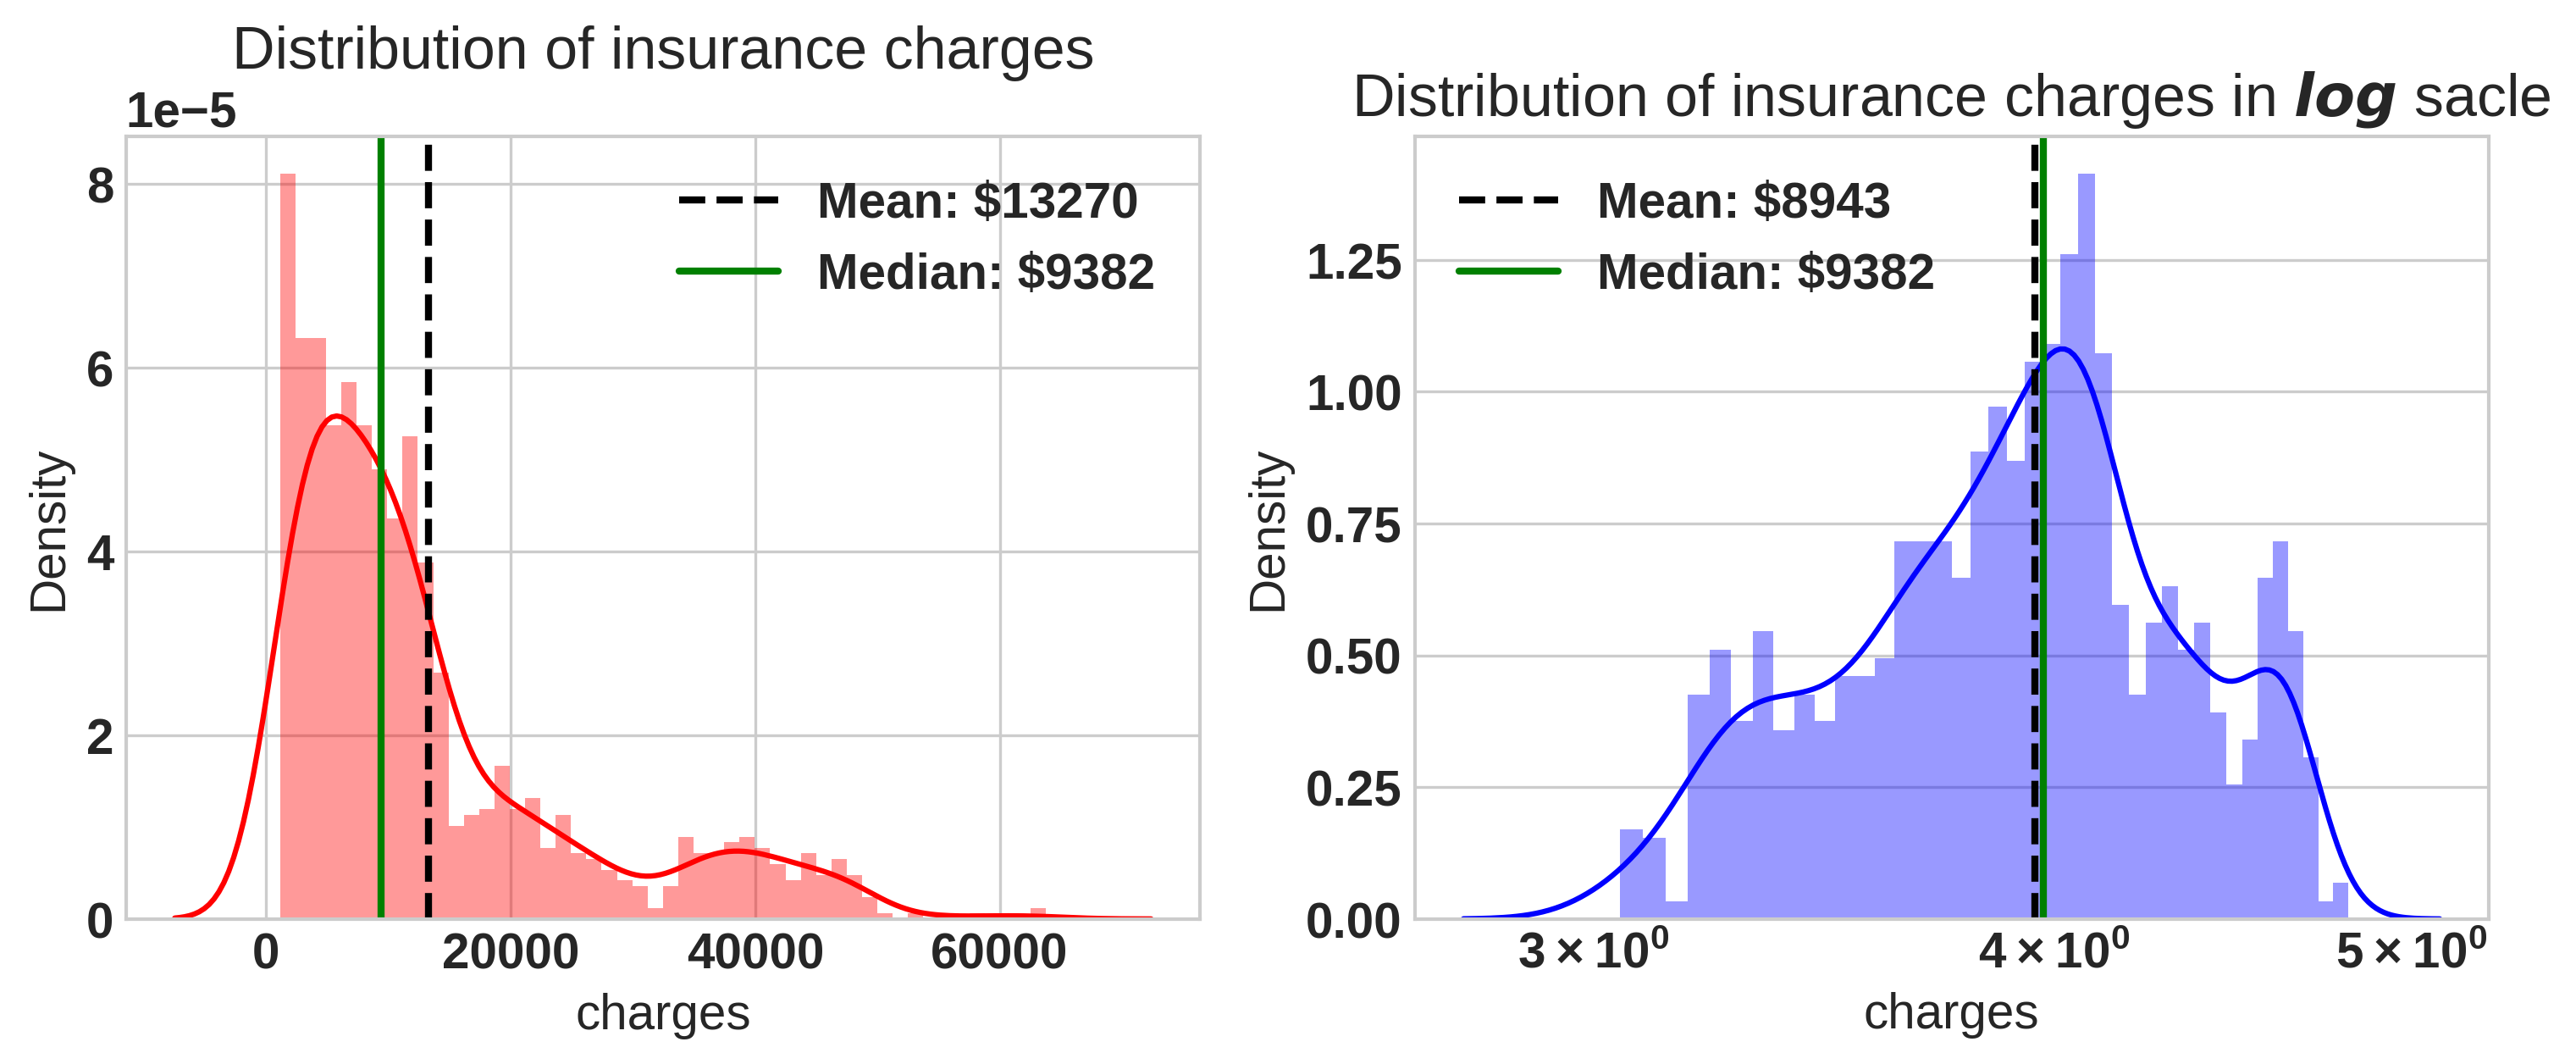
\includegraphics[width=0.9\textwidth]{charges_distribution.png}
\caption{Distribution of insurance charges showing right-skewed pattern (left) and log-transformed distribution (right)}
\label{fig:charges_distribution}
\end{figure}

\subsubsection{Correlation Analysis}
The correlation heatmap reveals no clear linear correlations between any features in the dataset, indicating minimal multicollinearity concerns. This is a positive finding as it means that features cannot be expressed as linear combinations of each other, suggesting that each predictor variable contributes unique information to the model. This independence between features supports the validity of using multiple linear regression without concerns about redundant predictors.

\begin{figure}[H]
\centering
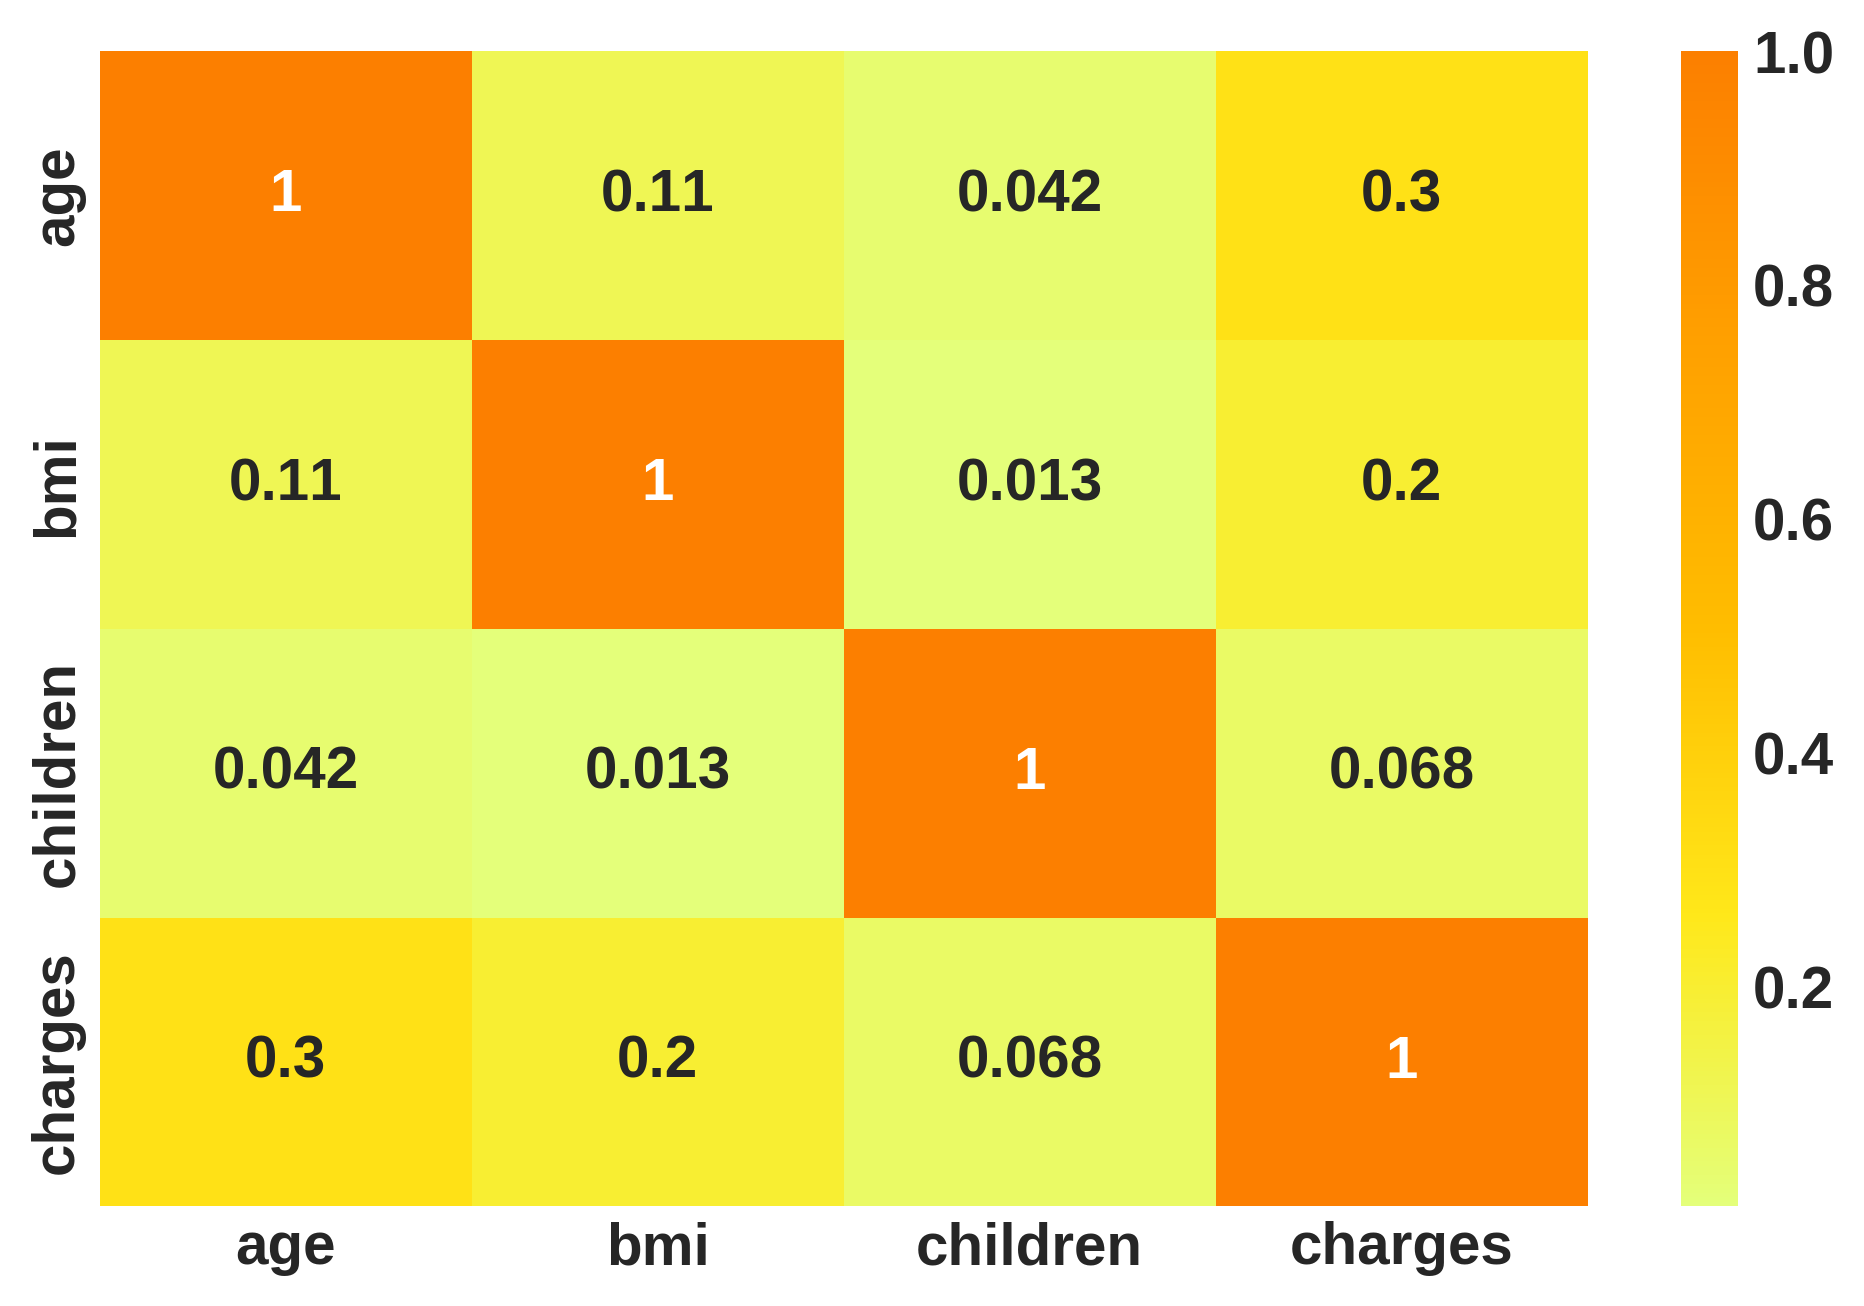
\includegraphics[width=0.8\textwidth]{correlation_heatmap.png}
\caption{Correlation matrix heatmap showing relationships between numerical variables}
\label{fig:correlation_heatmap}
\end{figure}

\newpage

\subsubsection{Feature-Target Relationship Analysis}

\textbf{Gender and Smoking Status Analysis}:

\begin{figure}[H]
\centering
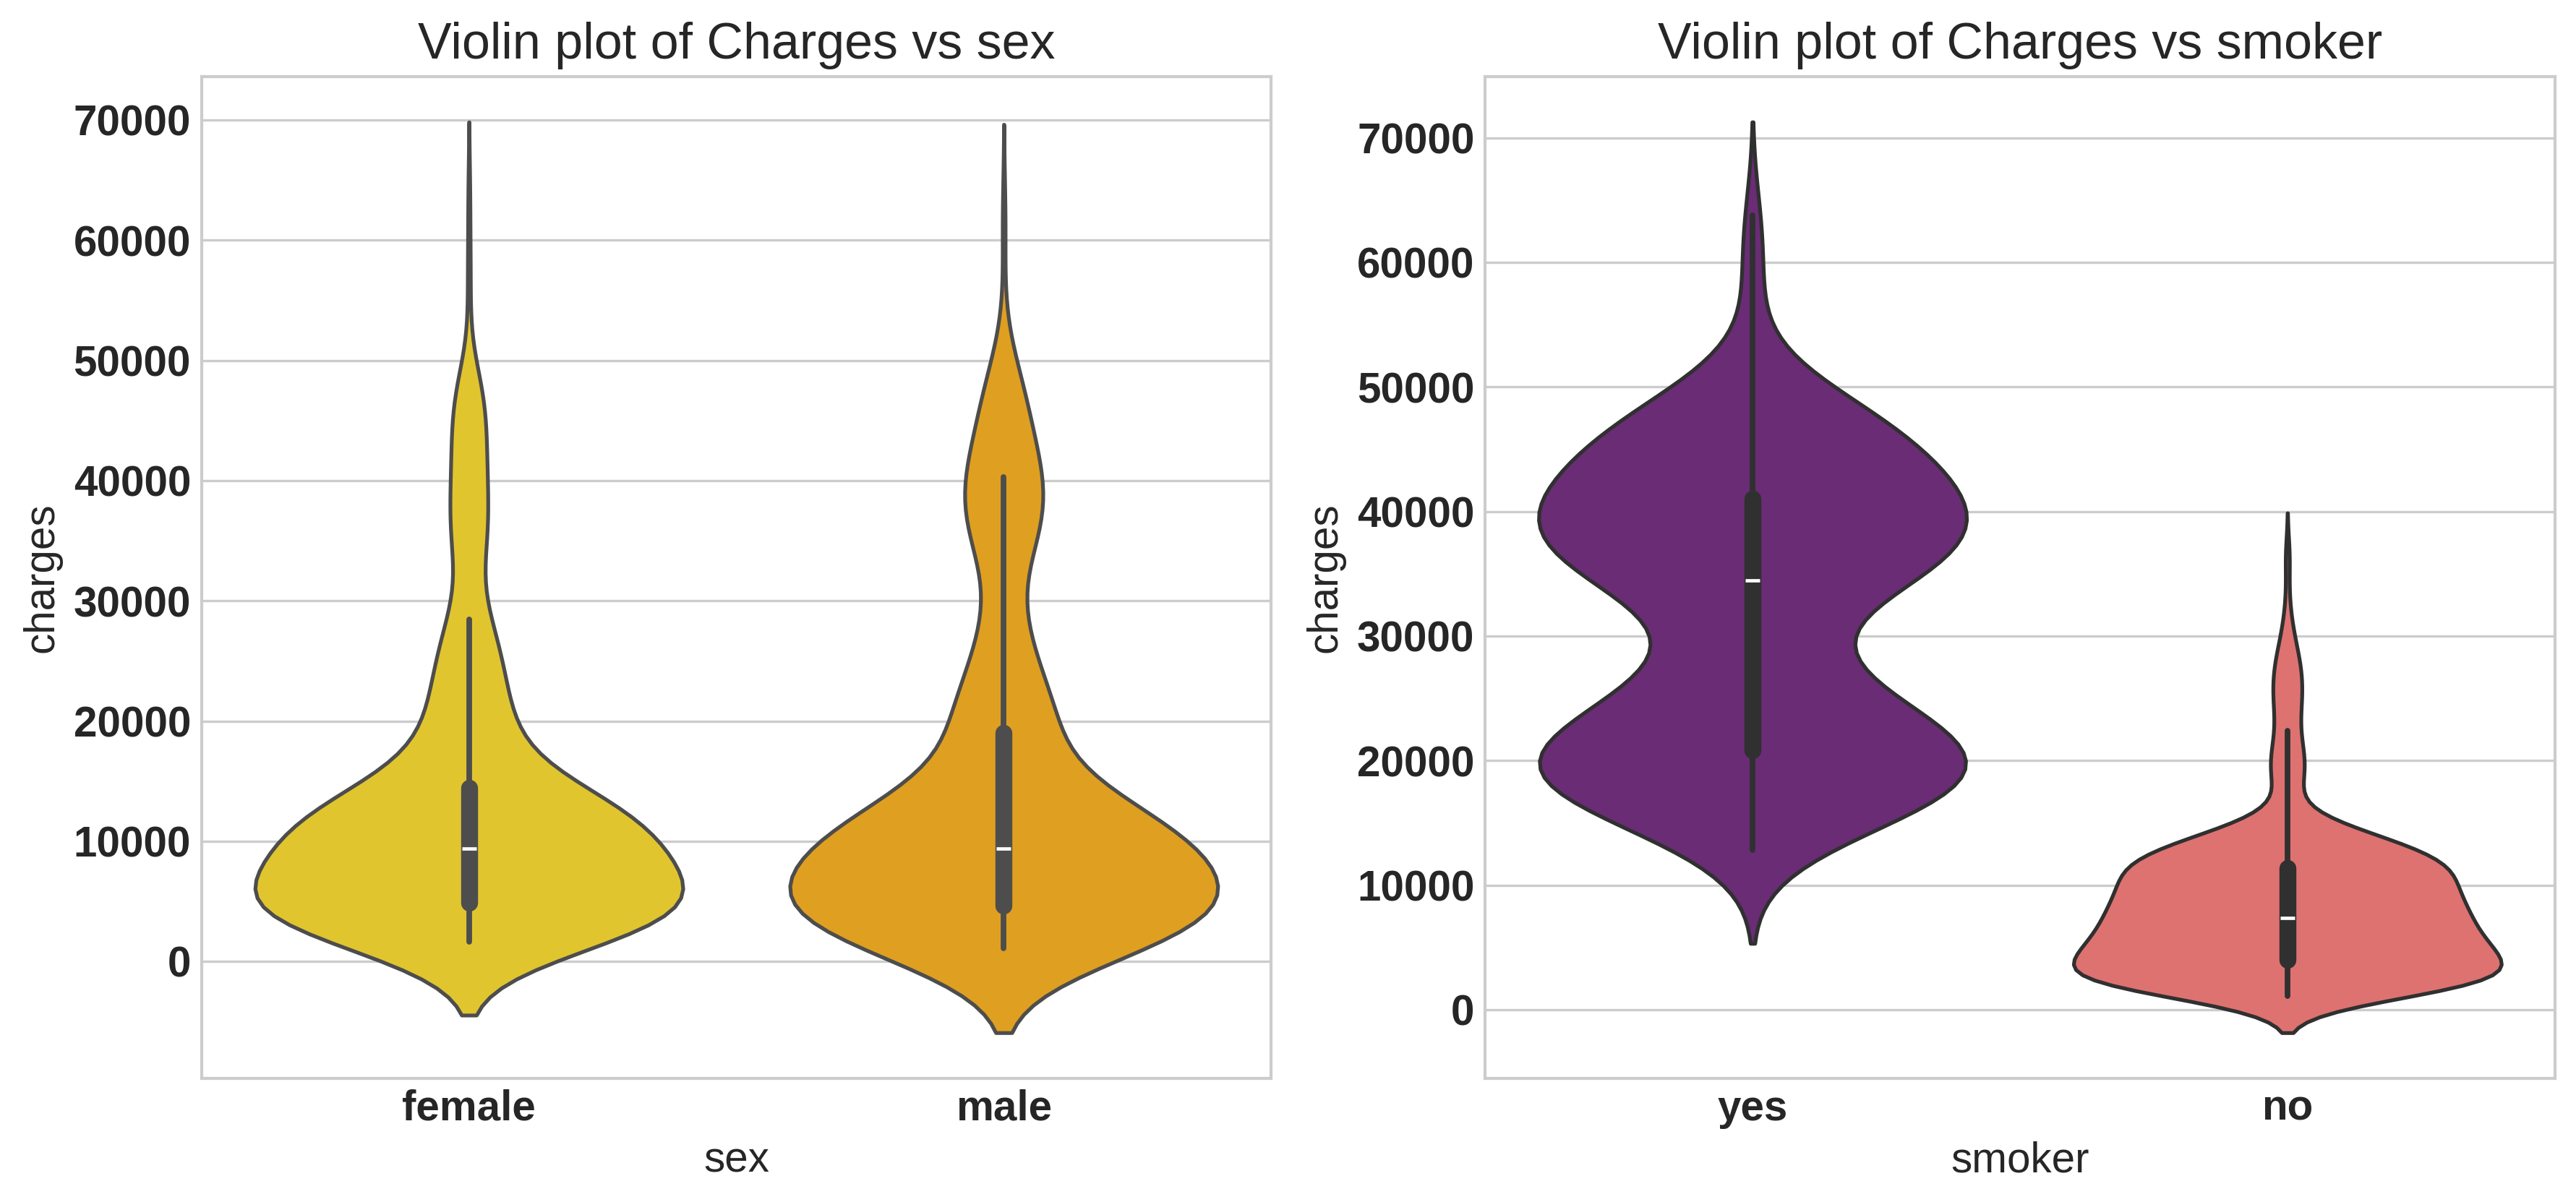
\includegraphics[width=0.9\textwidth]{violin_plots_sex_smoker.png}
\caption{Violin plots showing charge distributions by sex and smoking status}
\label{fig:violin_plots_sex_smoker}
\end{figure}

\textbf{Male vs Female}: The violin plots reveal that the spread and width of charge distributions for males and females are remarkably similar. Both groups are roughly centered around the same value, indicating that gender has minimal impact on insurance charges. This finding suggests that insurance pricing in this dataset is largely gender-neutral.

\textbf{Smoking Status}: The contrast between smokers and non-smokers is dramatic. Non-smokers exhibit a violin plot with a lower center and smaller width, while smokers show not only a wider distribution but are centered at much higher costs. This stark difference implies that smoking status has an extremely high impact on insurance charges, making it likely the most significant predictor in the dataset.

\textbf{BMI Relationship Analysis}:

\begin{figure}[H]
\centering
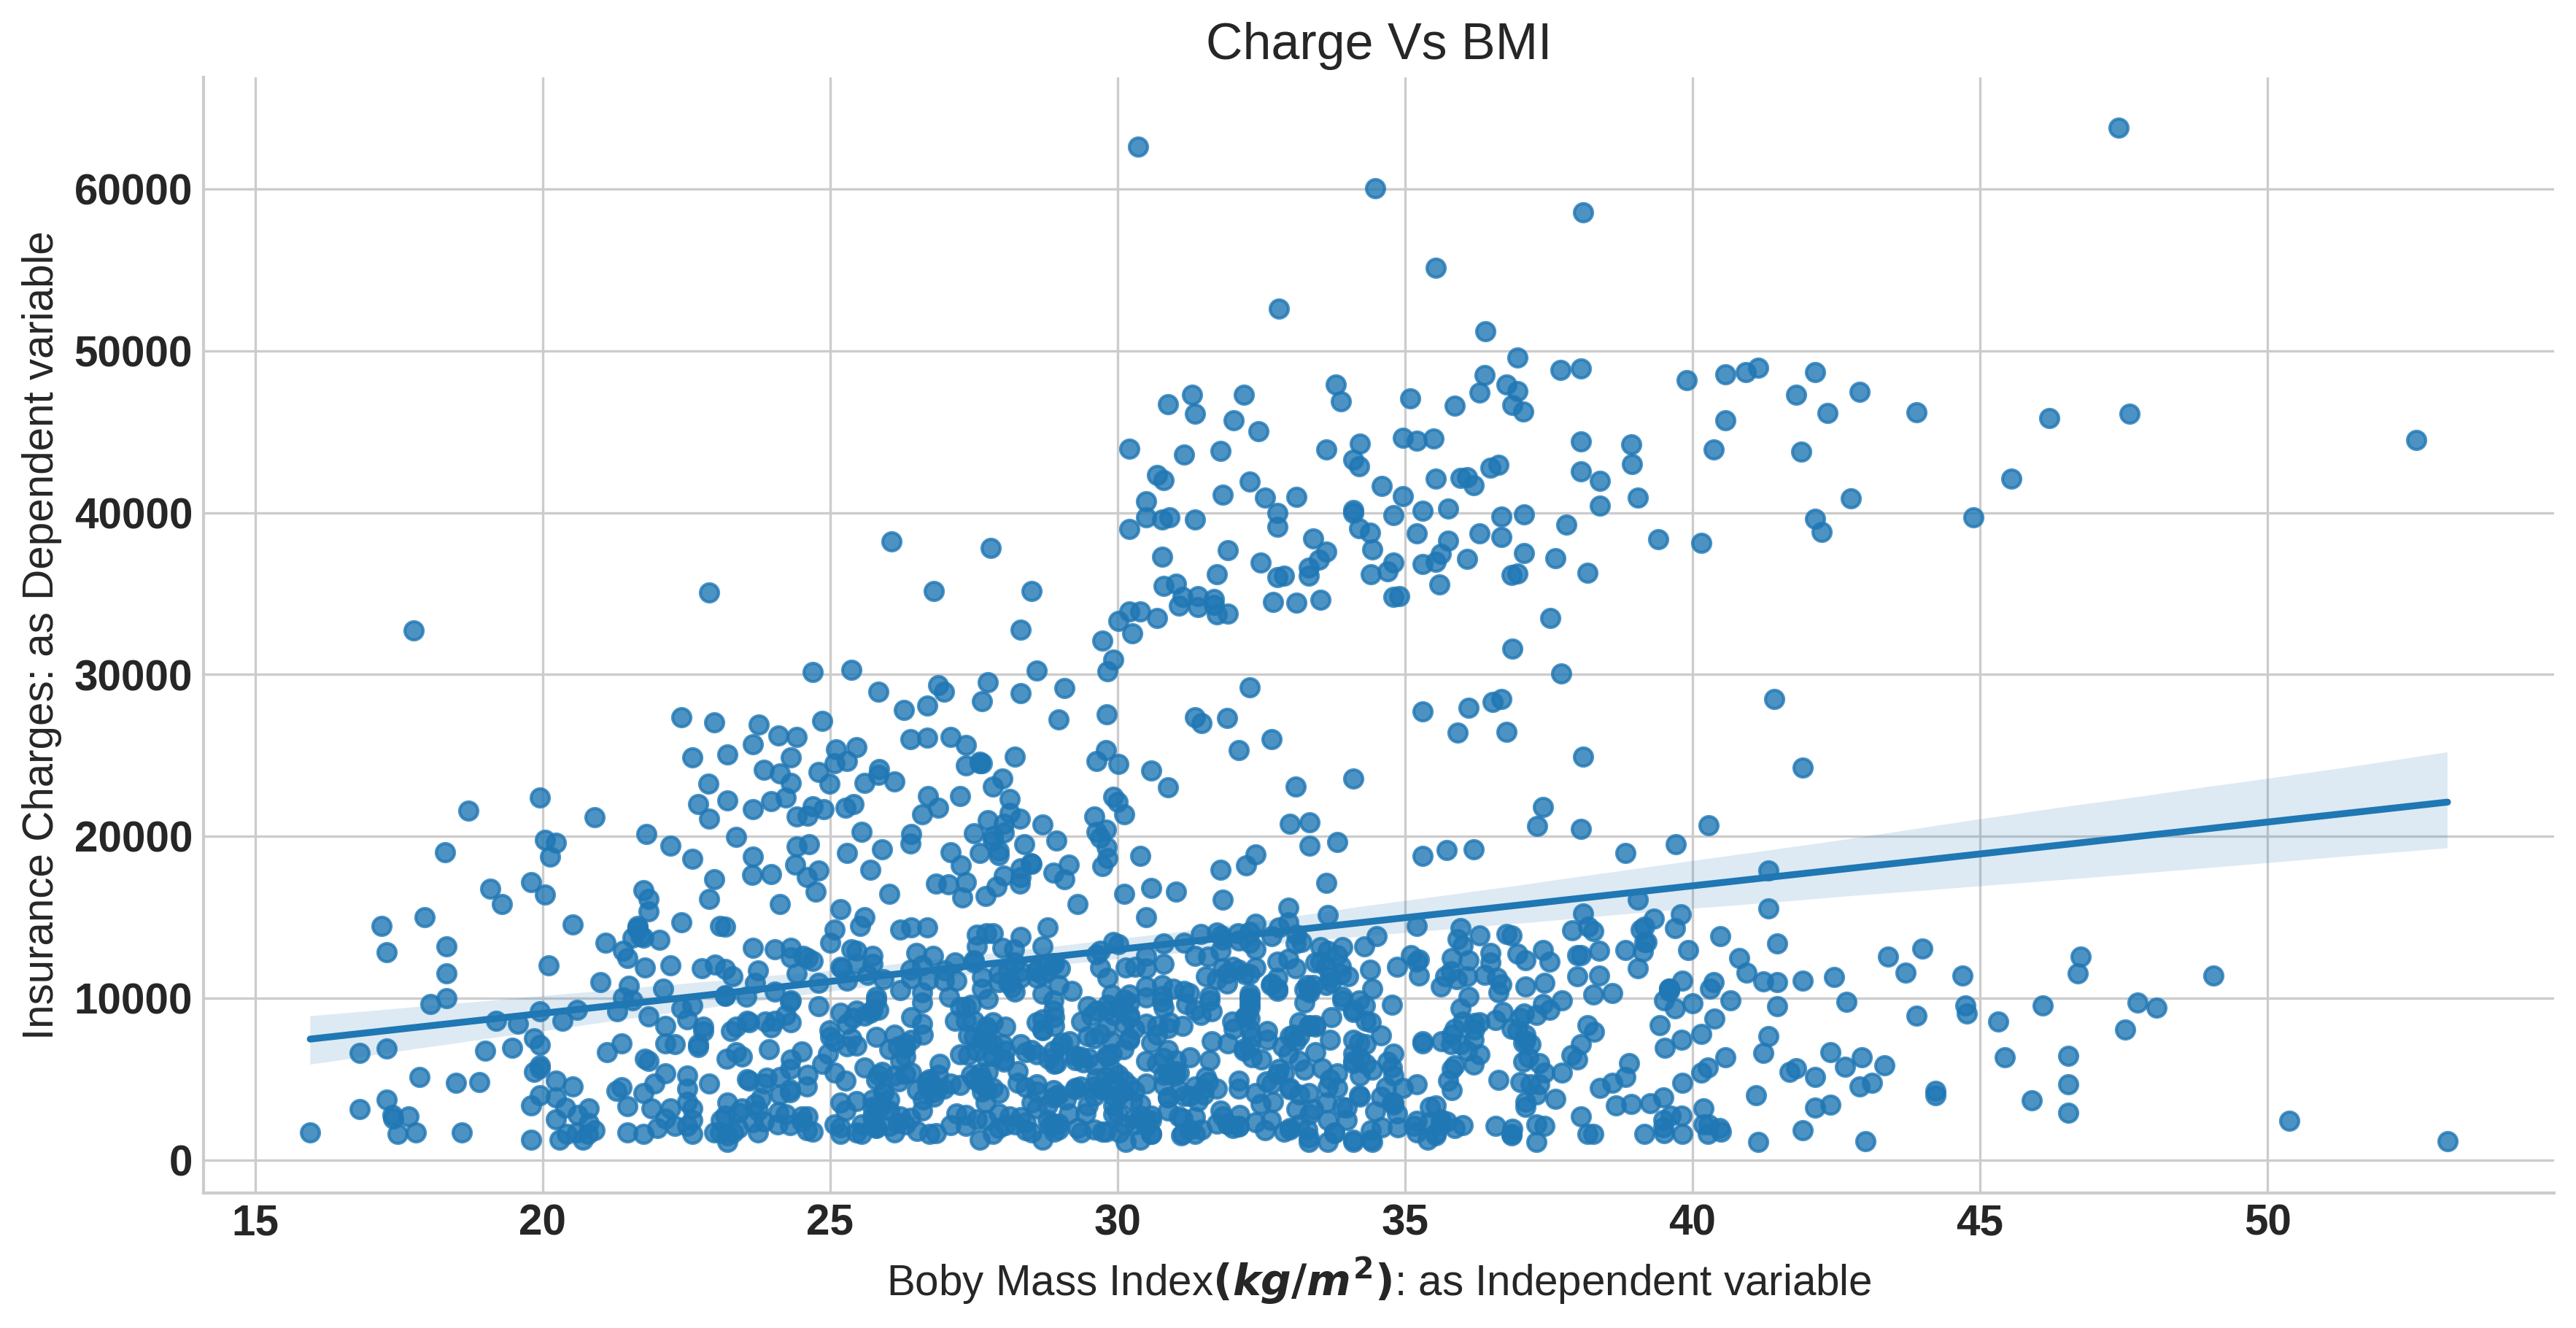
\includegraphics[width=0.8\textwidth]{charges_vs_bmi.png}
\caption{Scatter plot showing the relationship between BMI and insurance charges}
\label{fig:charges_vs_bmi}
\end{figure}

The BMI vs charges scatter plot reveals very noisy data but shows a small positive relationship between BMI and charges. However, this relationship appears to be more complex than a simple linear association, with smoking status acting as a significant modifier of the BMI effect.

\textbf{Children Analysis}:

\begin{figure}[H]
\centering
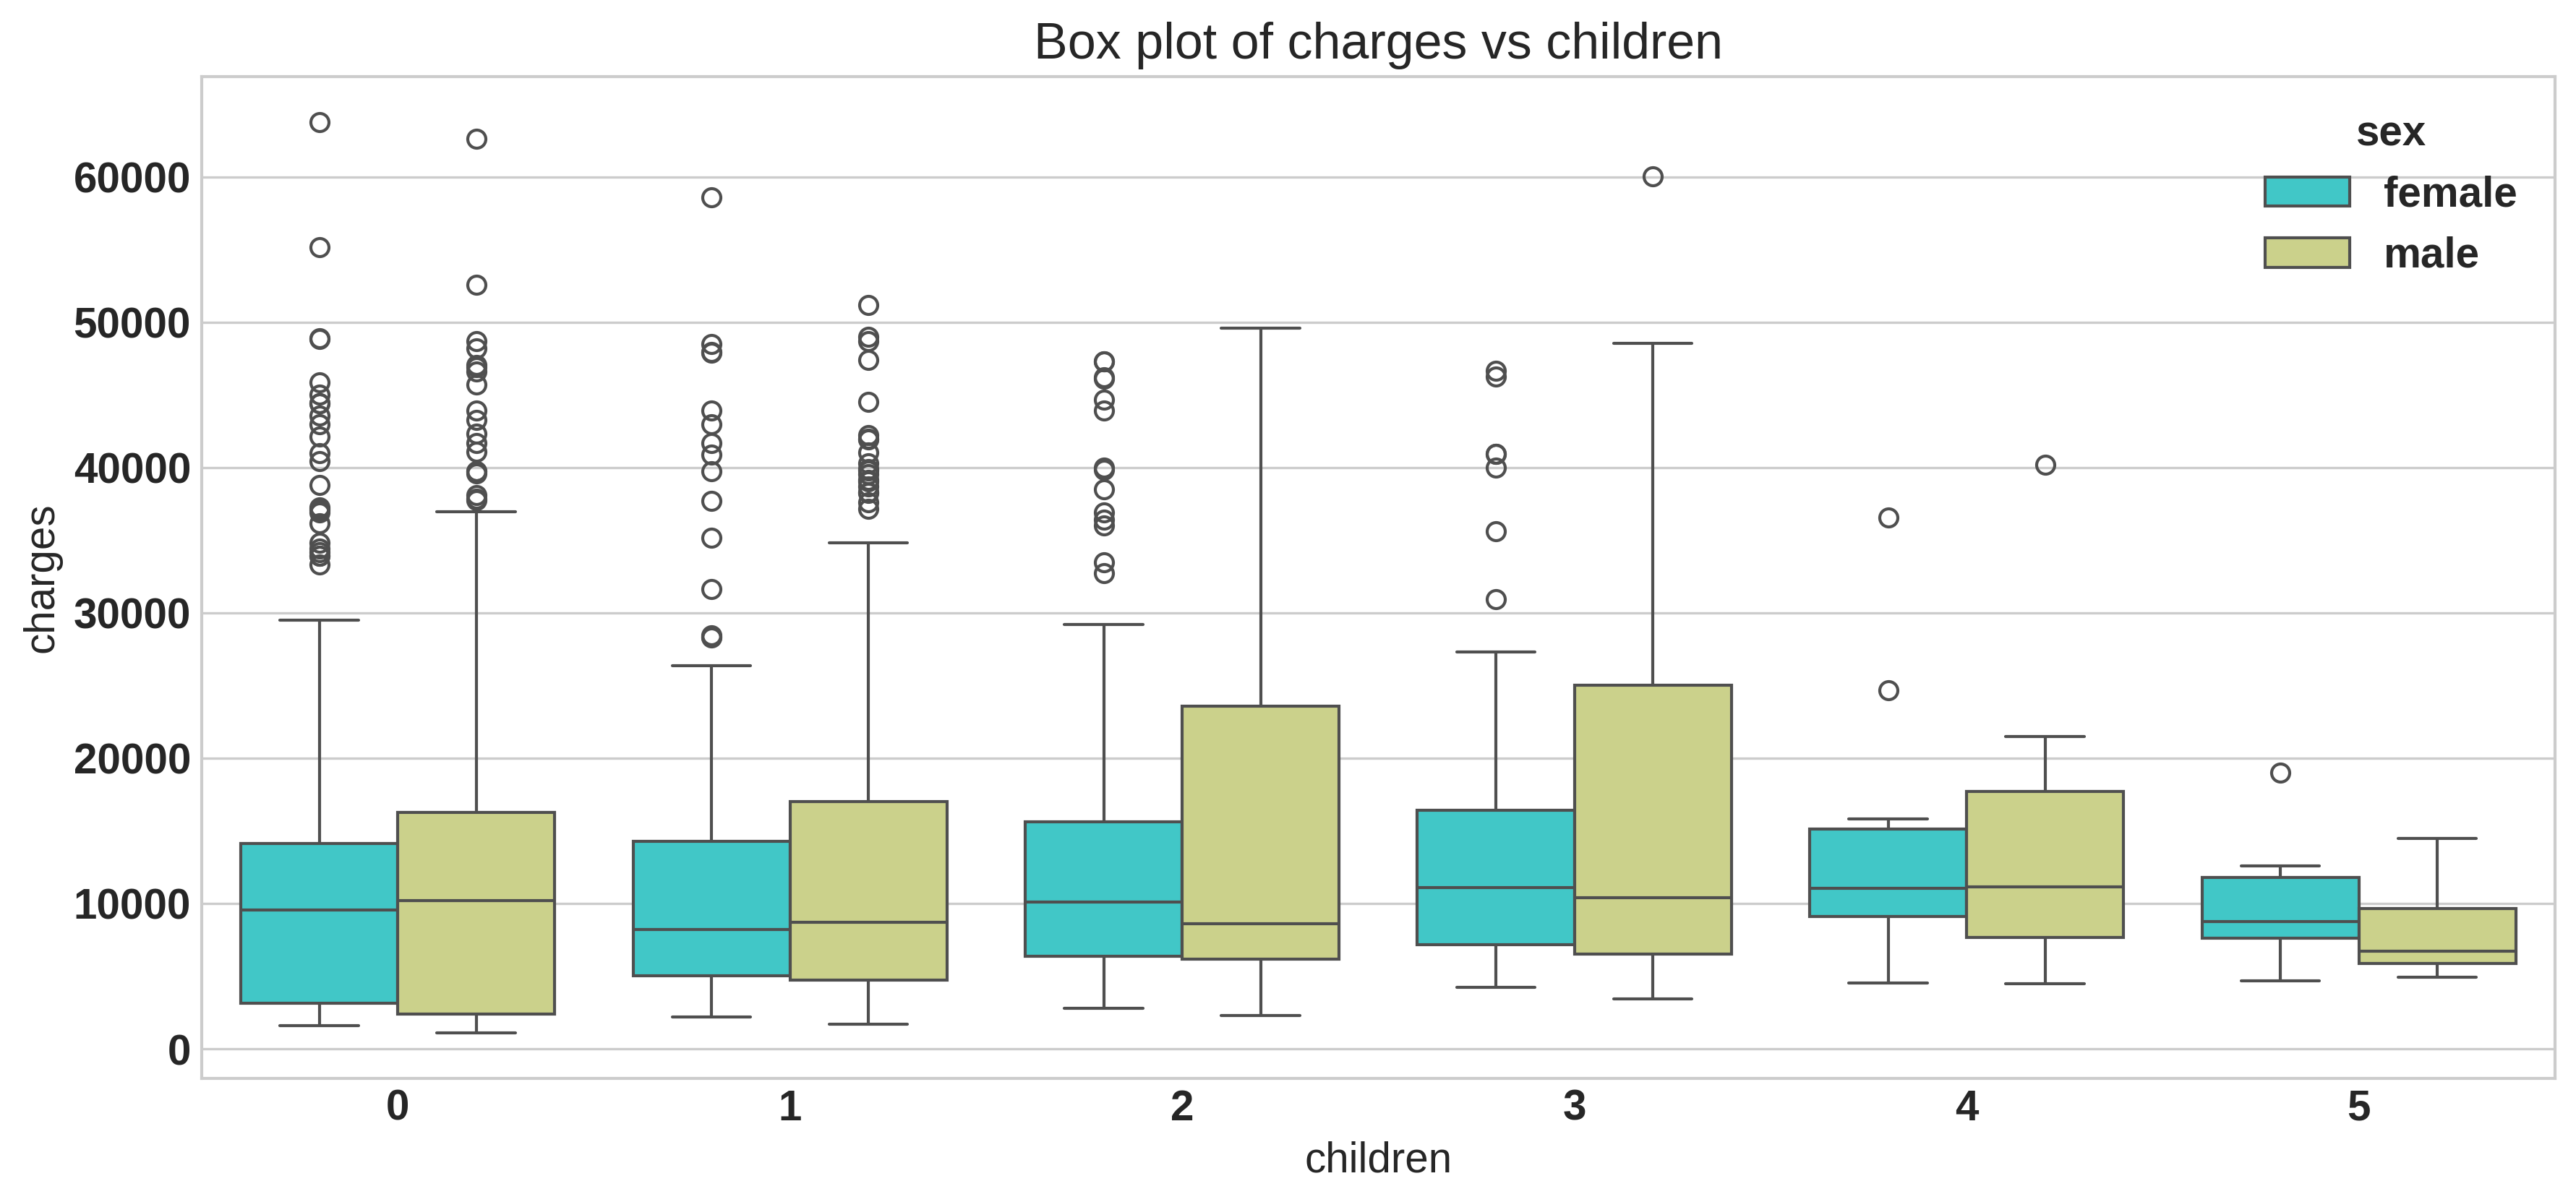
\includegraphics[width=0.9\textwidth]{boxplot_charges_vs_children.png}
\caption{Box plots showing charge distributions by number of children and sex}
\label{fig:boxplot_charges_vs_children}
\end{figure}

\begin{figure}[H]
\centering
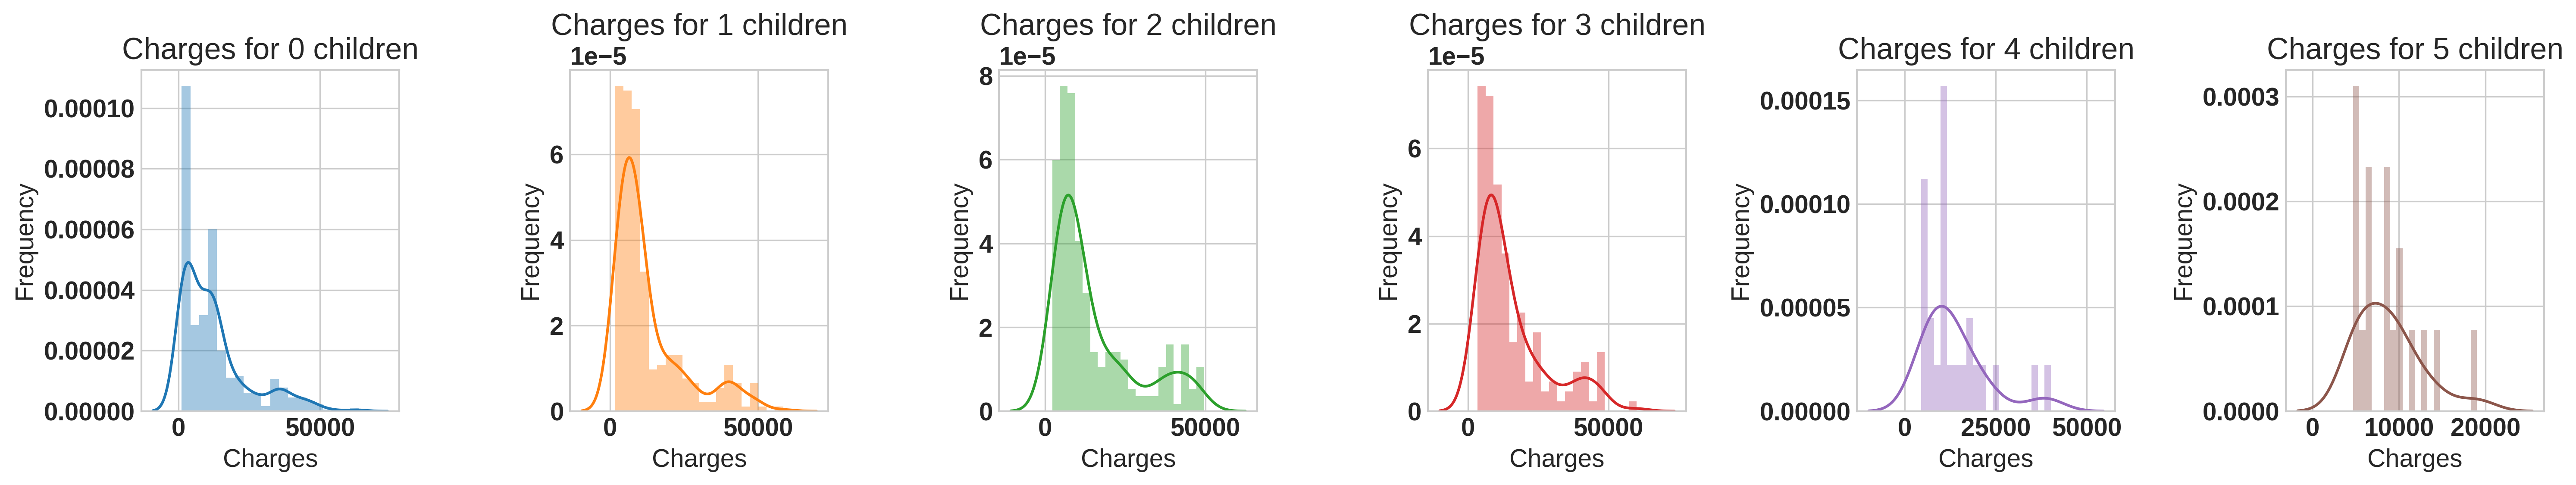
\includegraphics[width=0.9\textwidth]{charges_distribution_by_children.png}
\caption{Distribution of charges segmented by number of children}
\label{fig:charges_distribution_by_children}
\end{figure}

\begin{figure}[H]
\centering
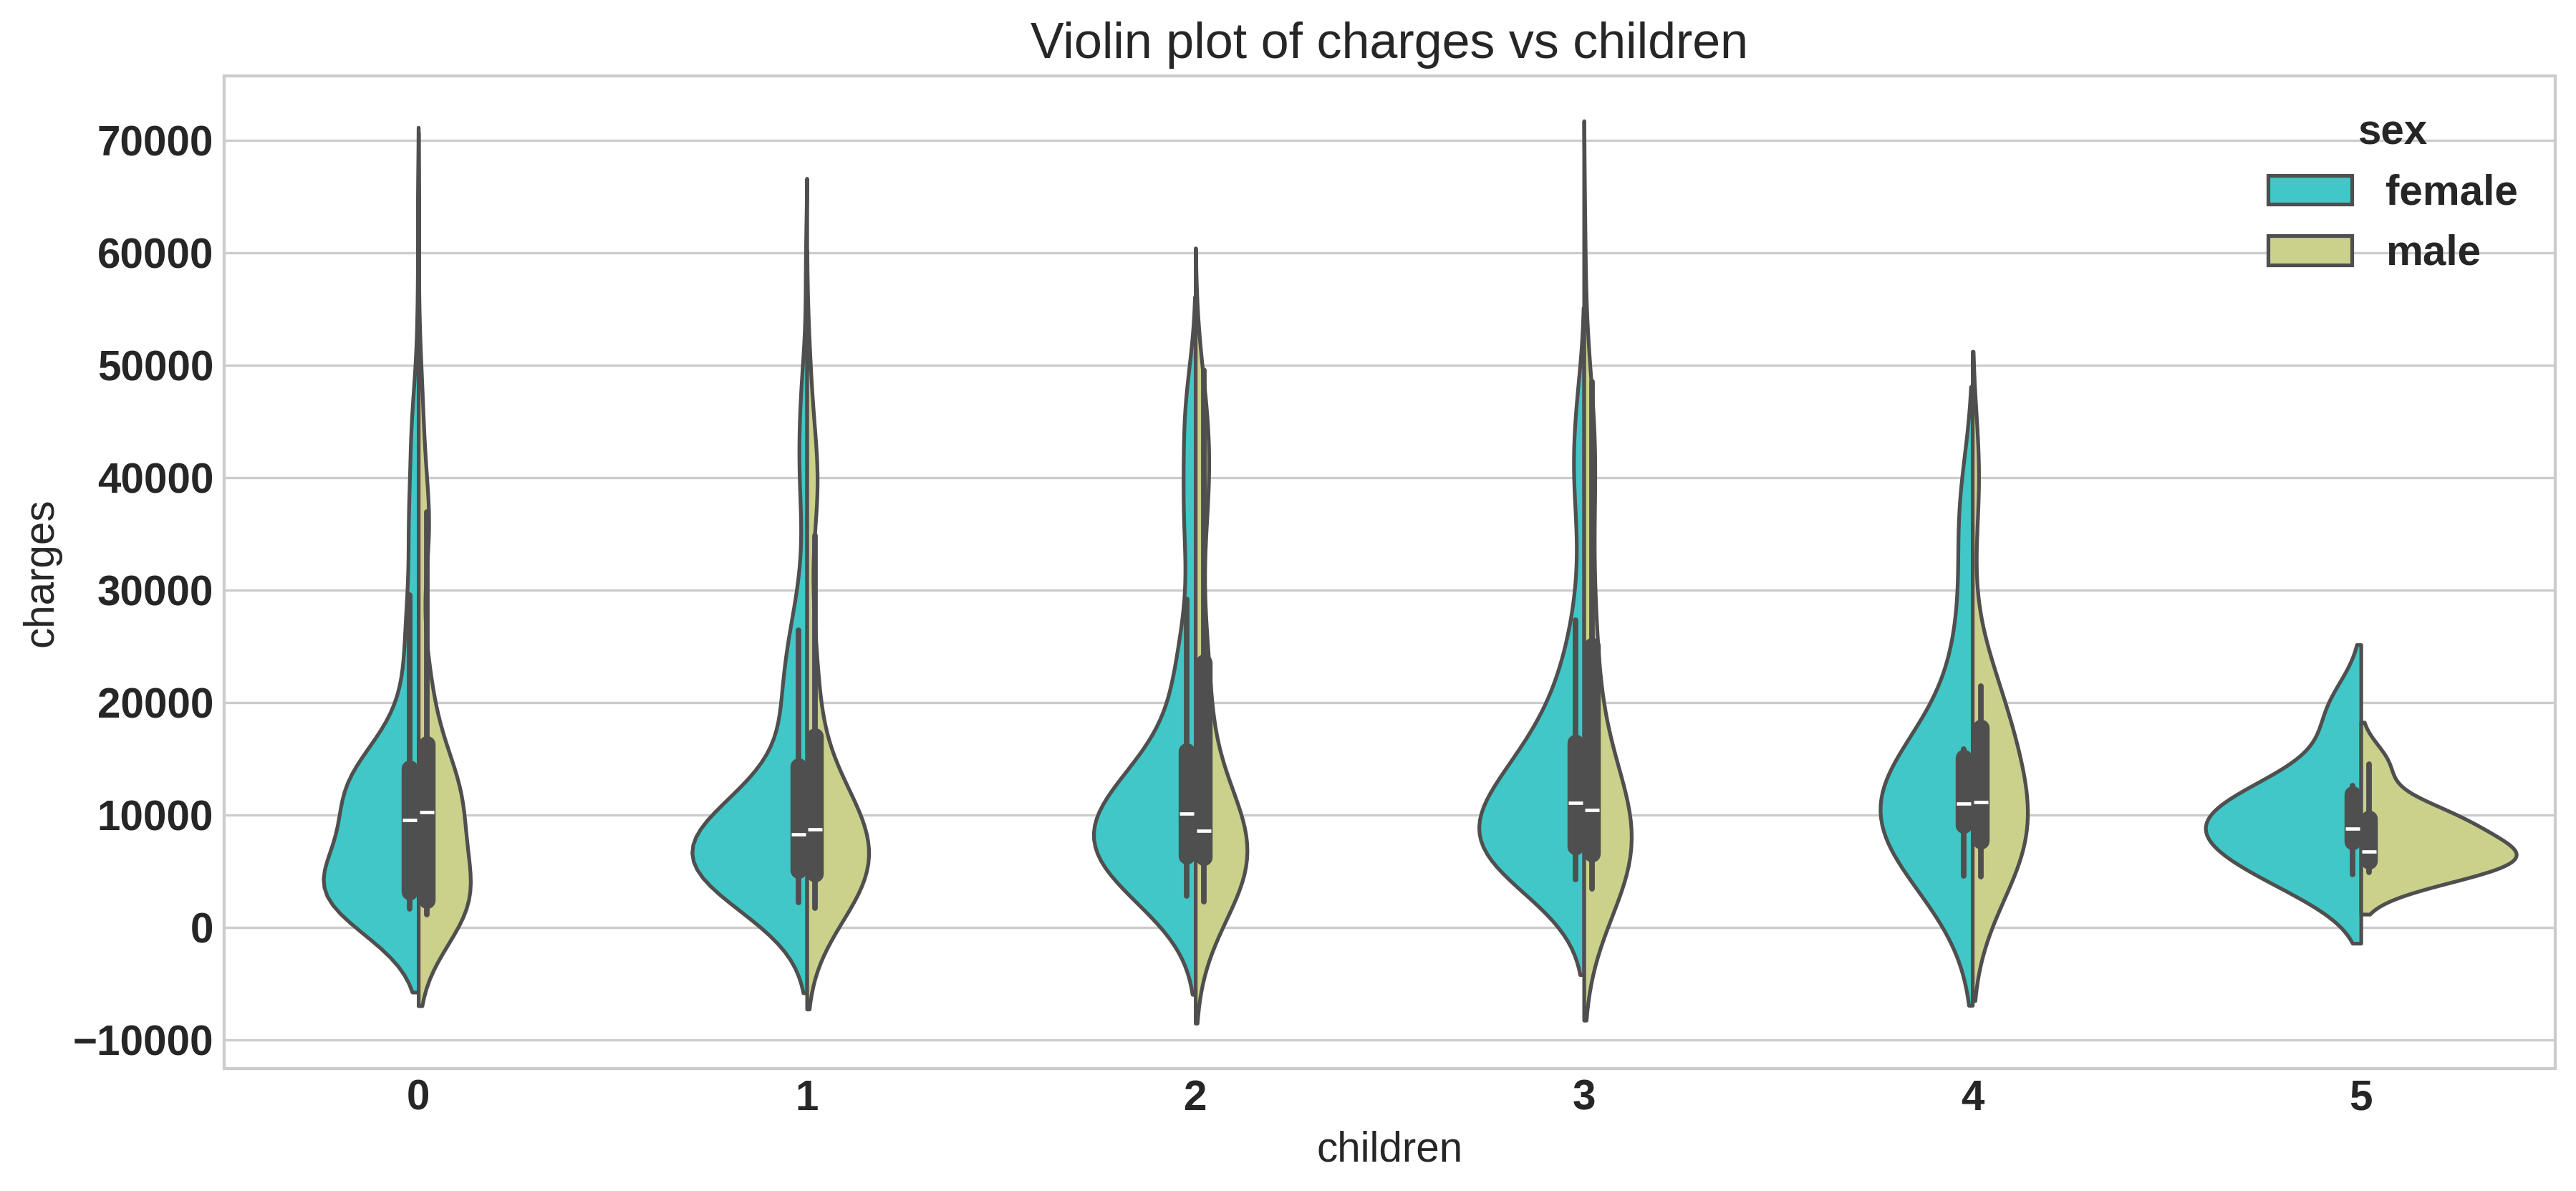
\includegraphics[width=0.9\textwidth]{violin_plot_charges_vs_children_by_sex.png}
\caption{Violin plots of charges vs children by sex}
\label{fig:violin_plot_charges_vs_children_by_sex}
\end{figure}

The analysis of charges by number of children reveals that the median charge is mostly centered around the same value regardless of family size. While families with 1, 2, or 3 children show higher spread in charges compared to those with 0, 4, or 5 children, this may be attributed to the distribution of family sizes in the dataset rather than a true effect of children count.

The violin plots demonstrate that charge distributions across different numbers of children are remarkably similar. The only noticeably smaller distribution is for families with 5 children, but this is likely due to the smaller sample size of such families in the dataset. This analysis suggests that the number of children is not a high-impact feature on insurance charges.

\textbf{Regional Analysis}:

\begin{figure}[H]
\centering
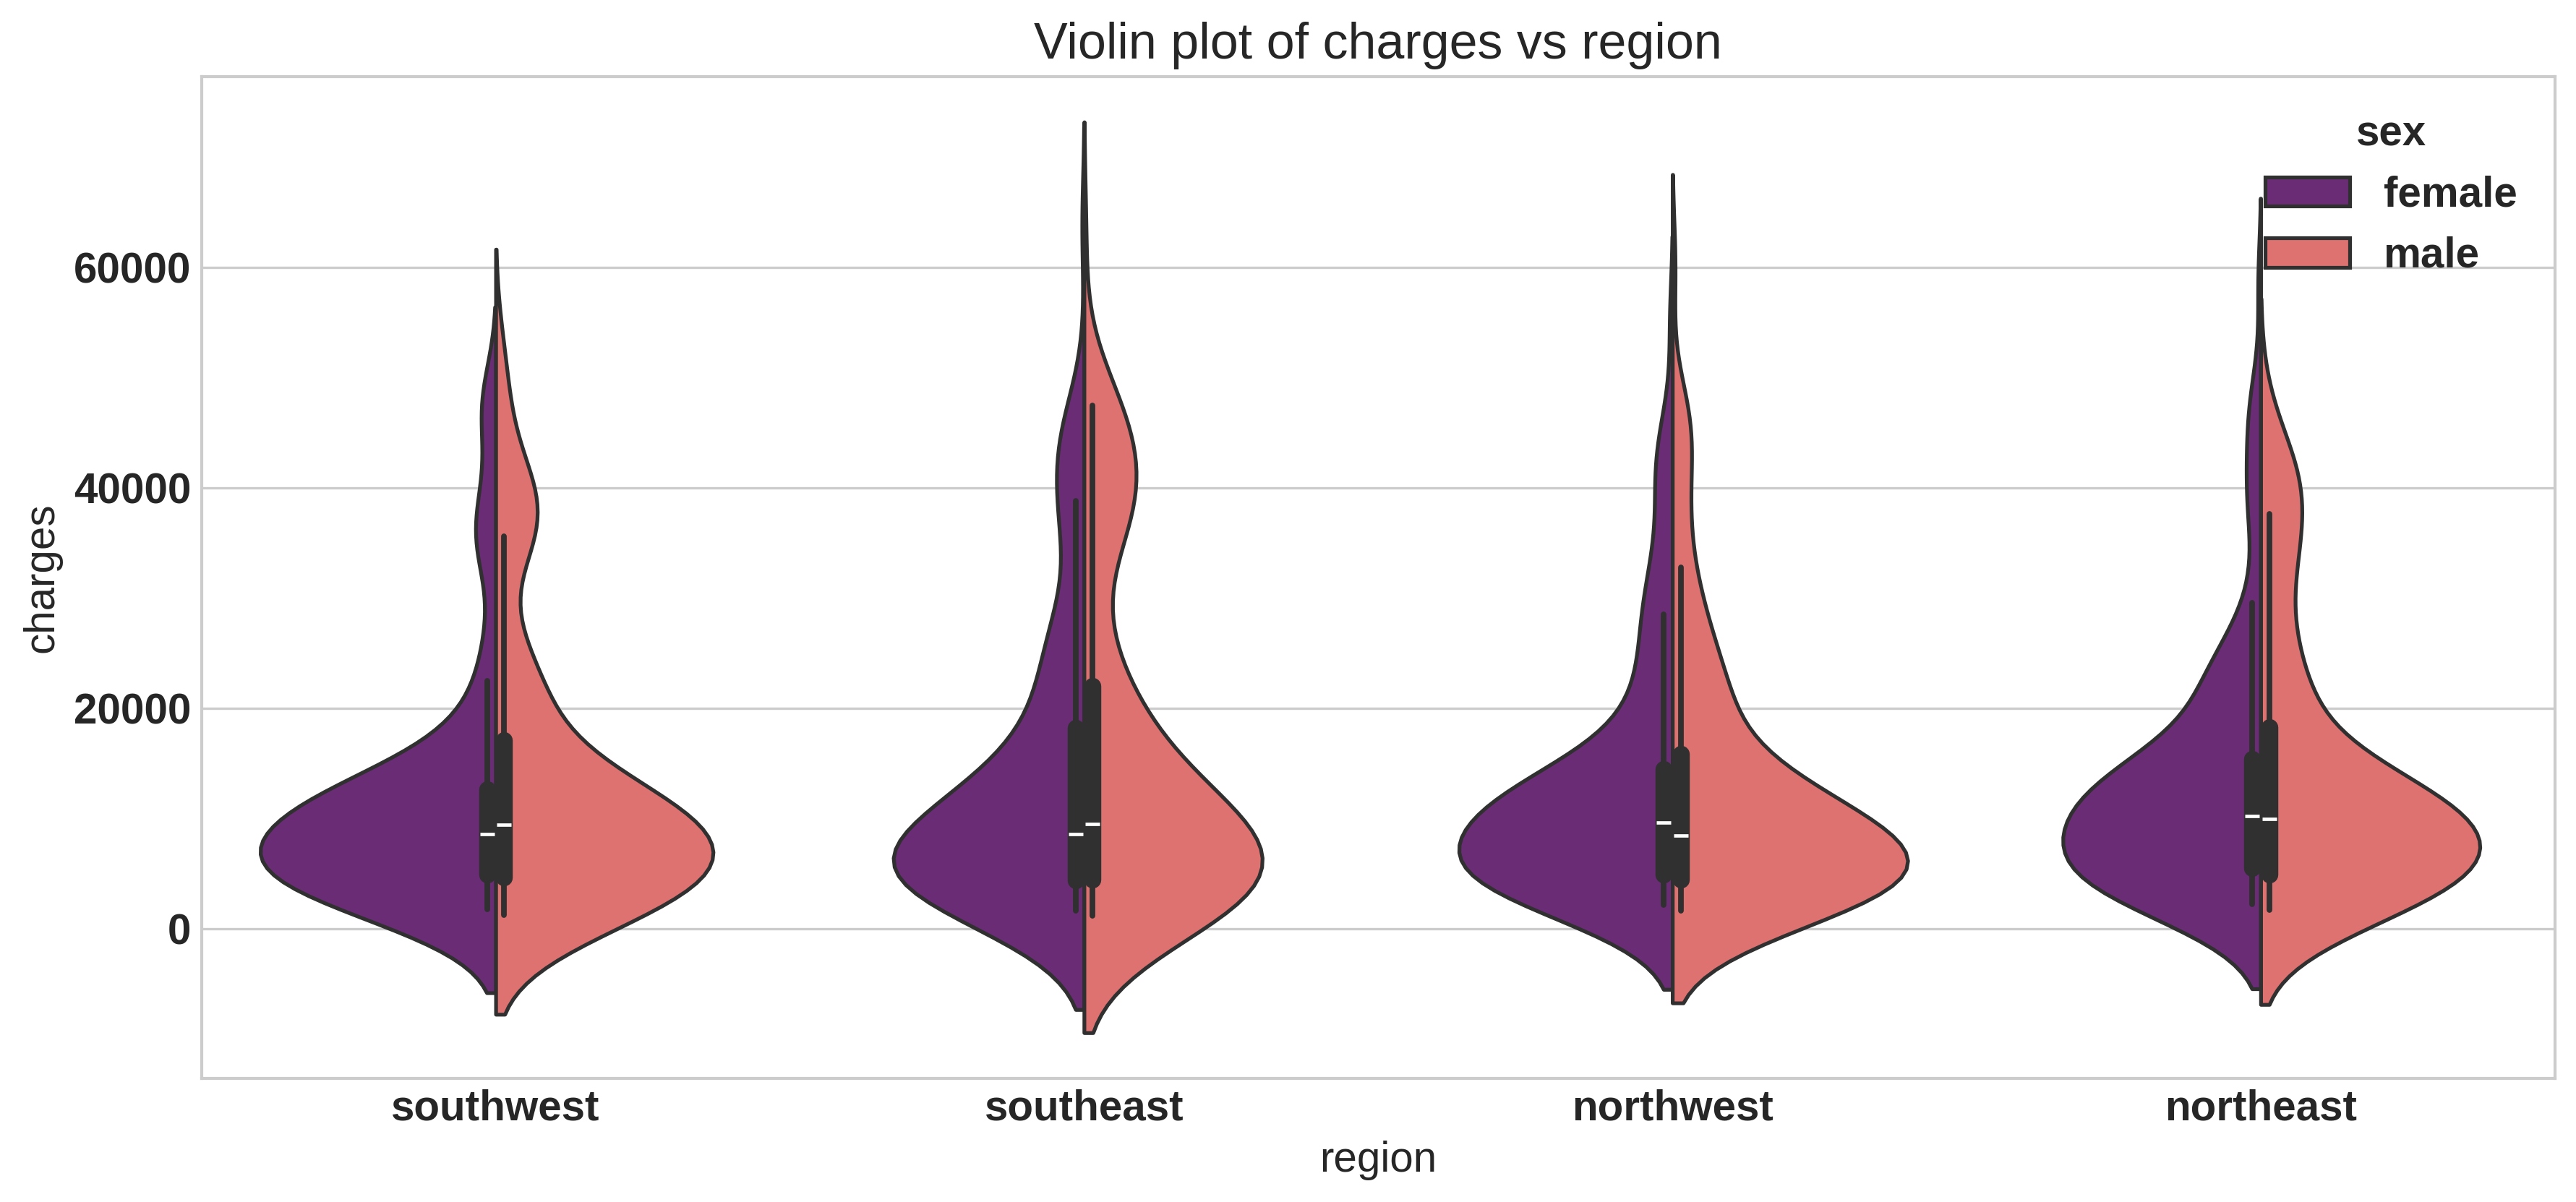
\includegraphics[width=0.9\textwidth]{violin_plot_charges_vs_region_by_sex.png}
\caption{Violin plots of charges vs region by sex}
\label{fig:violin_plot_charges_vs_region_by_sex}
\end{figure}

The violin plots for each geographical region appear extremely similar in both width and stretch, and are centered near the same value. This similarity across regions suggests that, like gender, geographical region does not have a high impact on insurance charges. This finding indicates that the insurance pricing strategy may be standardized across different regions.

\subsubsection{Interaction Effects Analysis}

\begin{figure}[H]
\centering
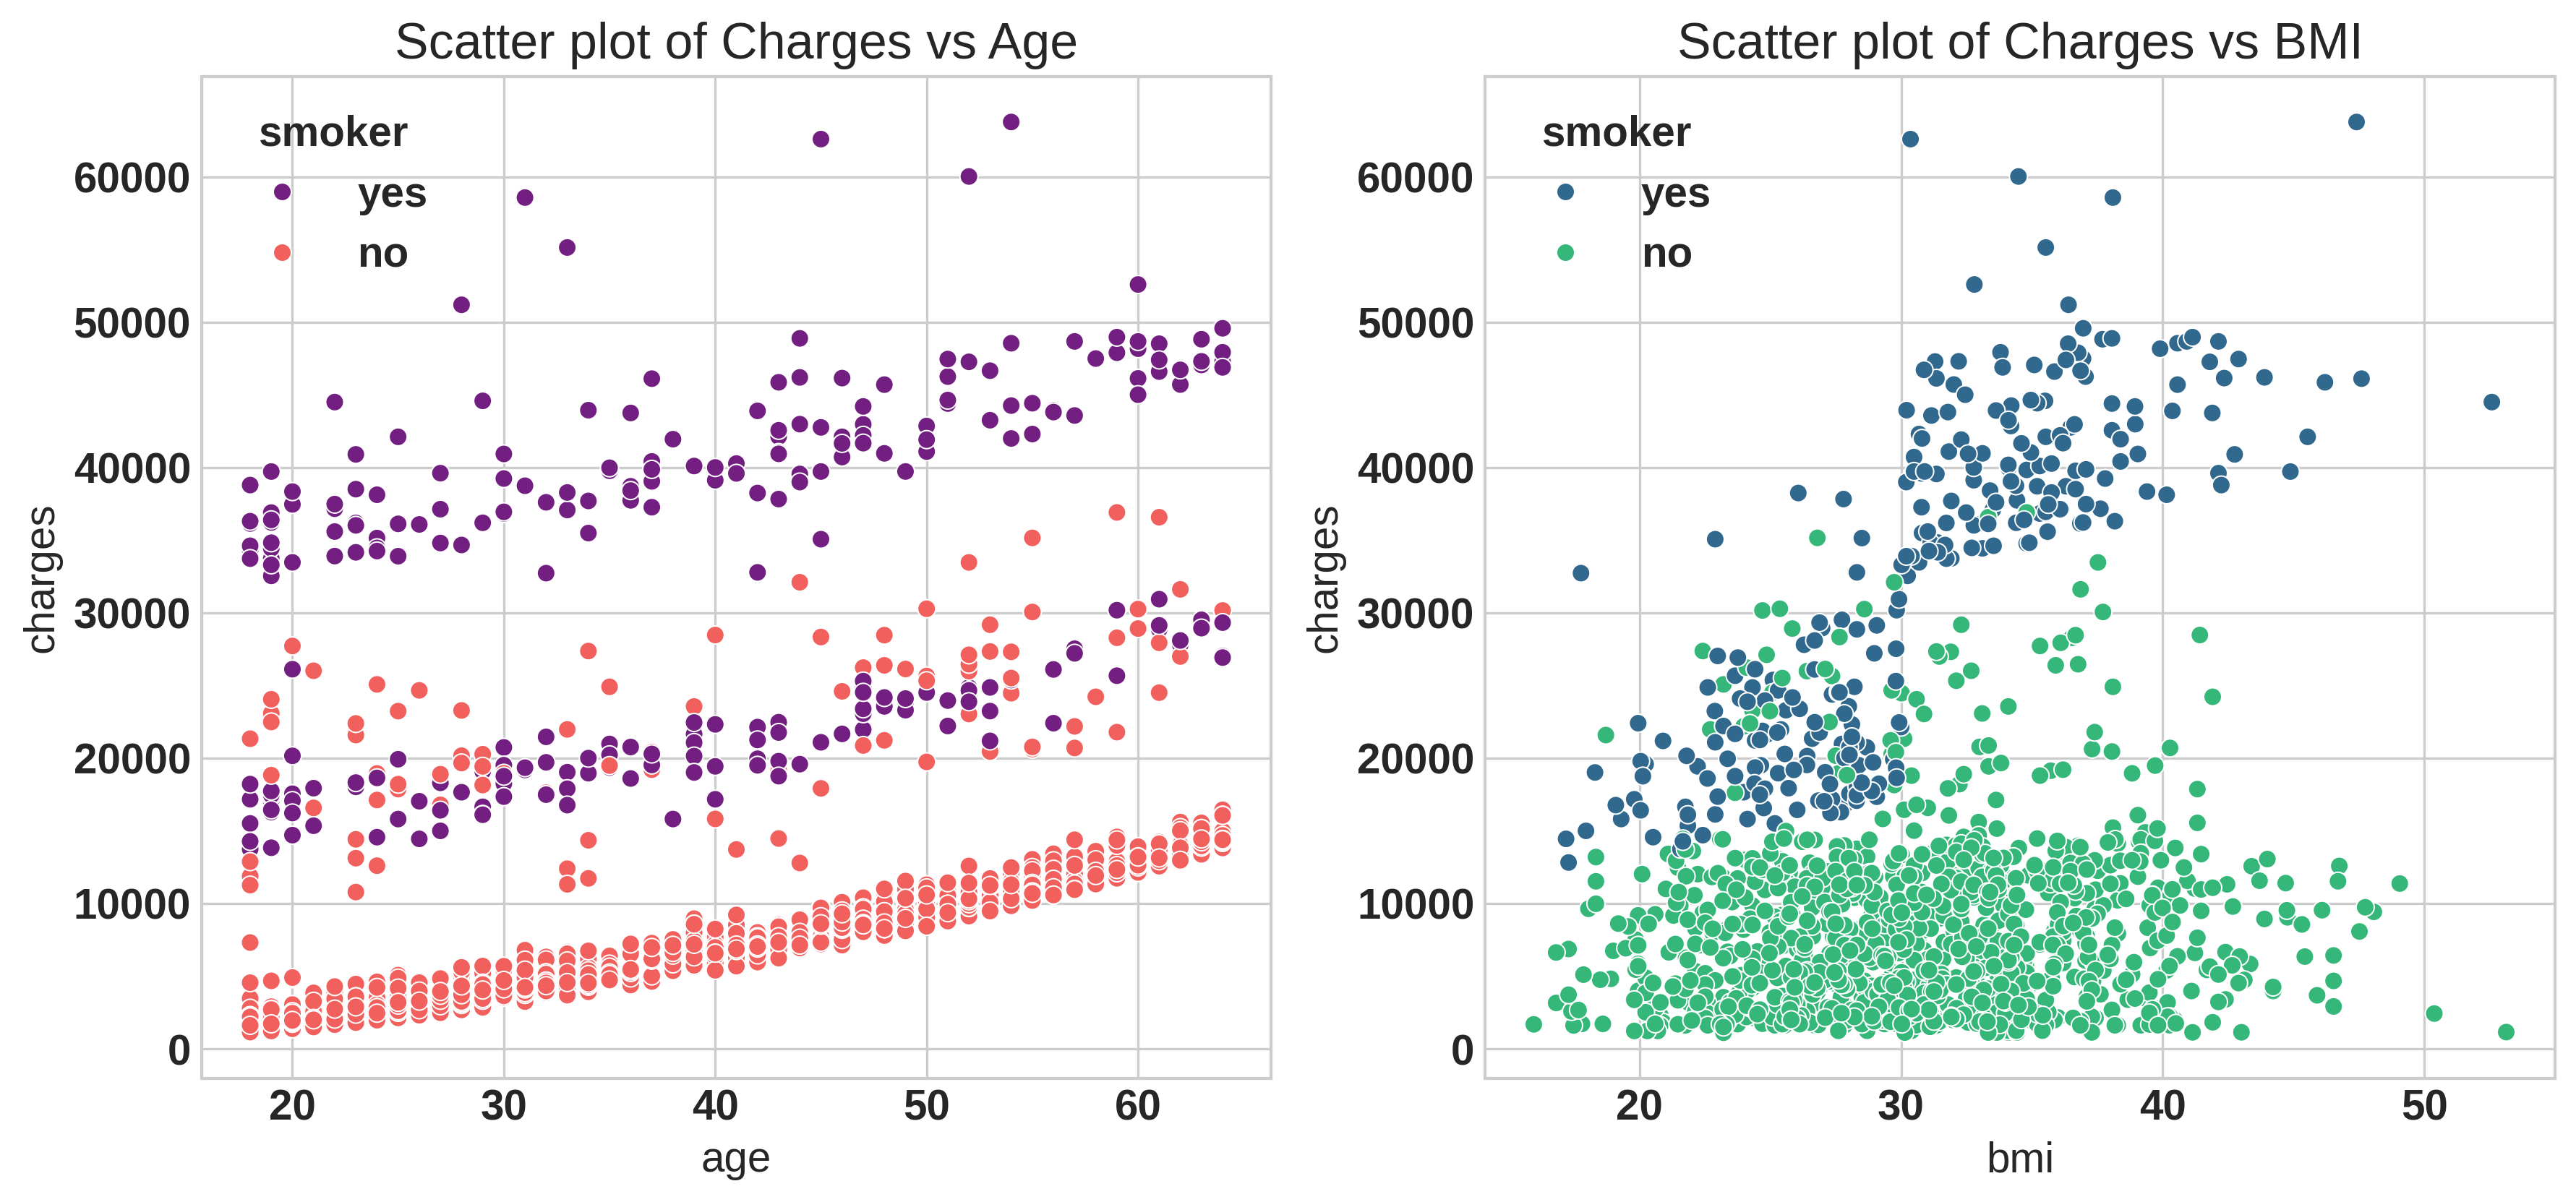
\includegraphics[width=0.9\textwidth]{scatter_plots_charges_vs_age_bmi.png}
\caption{Scatter plots showing interactions between age/BMI and smoking status on charges}
\label{fig:scatter_plots_charges_vs_age_bmi}
\end{figure}

\textbf{Age, Smoking, and Charges Interaction}:
The age vs charges scatter plot reveals three distinct levels of charges:
\begin{enumerate}
    \item \textbf{First level}: Non-smokers with relatively healthy profiles - representing baseline charges for average healthy individuals
    \item \textbf{Second level}: Either smokers with lower risk profiles or non-smokers with other risk factors - suggesting moderate risk pricing
    \item \textbf{Third level}: High-risk smokers - representing premium charges for the highest risk category
\end{enumerate}

This three-tier structure suggests hidden complexity in the data that may not be fully captured by simple additive models. Factors such as activity level (inactive non-smokers potentially falling into the second level) or smoking intensity (heavy smokers vs. light smokers) may create correlations between supposedly distinct groups.

\textbf{BMI and Smoking Interaction}:
The BMI vs charges plot provides crucial insight into the third tier observed in the age analysis. At lower BMI values (20-30), there is a noticeable but moderate disparity between smokers and non-smokers. However, at higher BMI values (30+), this disparity grows significantly, creating a substantial gap between non-smokers and smokers with high BMI.

This interaction effect suggests that the highest charge category consists primarily of high BMI smokers, representing individuals at the greatest risk for health issues. The multiplicative effect of smoking and high BMI creates a compounding risk profile that justifies premium pricing.

\subsection{Model Development}

\subsubsection{Linear Regression}
A multiple linear regression model was initially fitted as the primary approach using all available predictors:
$$\hat{y} = \beta_0 + \beta_1 \cdot \text{age} + \beta_2 \cdot \text{sex} + \beta_3 \cdot \text{BMI} + \beta_4 \cdot \text{children} + \beta_5 \cdot \text{smoker} + \beta_6 \cdot \text{region}$$

This baseline model served as the foundation for understanding the relationships between predictors and insurance charges.

\subsubsection{Ridge Regression}  
Following the initial linear regression analysis, Ridge regression with L2 regularization was implemented:
$$\min_{\boldsymbol{\beta}} \left\{ \frac{1}{n}\sum_{i=1}^{n}(y_i - \mathbf{x}_i^T\boldsymbol{\beta})^2 + \lambda\|\boldsymbol{\beta}\|_2^2 \right\}$$

Regularization paths were analyzed across different alpha values (1 to 99) to understand coefficient behavior under varying regularization strengths and to validate the stability of the linear regression findings.

\subsubsection{Why Ridge?}
Given the large value of the Smoker coefficient observed in the initial linear regression model:
Ridge regression was employed to check the weights and stabilize the coefficients to prevent potential overfitting. After analyzing the regularization paths, it was found that the Smoker coefficient was reduced to 14,374.39, which is still significantly larger than the other coefficients, confirming the robustness of this finding.

\subsection{Model Diagnostics}

Several diagnostic tests were performed to validate model assumptions:
\begin{itemize}
    \item \textbf{Linearity}: Assessed through actual vs. predicted value scatter plots
    \item \textbf{Residual Normality}: Evaluated using distribution plots and Q-Q plots
    \item \textbf{Variance Inflation Factor}: Calculated to assess multicollinearity
\end{itemize}

\section{Analysis Results}

\subsection{Model Performance}

The linear regression model achieved the following performance metrics:
\begin{itemize}
    \item \textbf{R-squared}: 0.7694 (76.94\% of variance explained)
    \item \textbf{Mean Squared Error}: 33,806,944
    \item \textbf{Variance Inflation Factor}: 4.33
\end{itemize}

These results indicate that the model explains approximately 77\% of the variance in insurance charges, representing good predictive performance for this type of analysis.

\subsection{Feature Importance Analysis}

The linear regression coefficients revealed the relative importance of different factors:

\begin{table}[H]
\centering
\begin{tabular}{lrr}
\toprule
\textbf{Feature} & \textbf{Coefficient} & \textbf{Absolute Value} \\
\midrule
Smoker & 23,644.44 & 23,644.44 \\
Children & 425.61 & 425.61 \\
BMI & 344.77 & 344.77 \\
Age & 261.17 & 261.17 \\
Region & 234.58 & 234.58 \\
Sex & 106.59 & 106.59 \\
\bottomrule
\end{tabular}
\caption{Feature importance based on linear regression coefficients}
\end{table}

\begin{figure}[H]
\centering
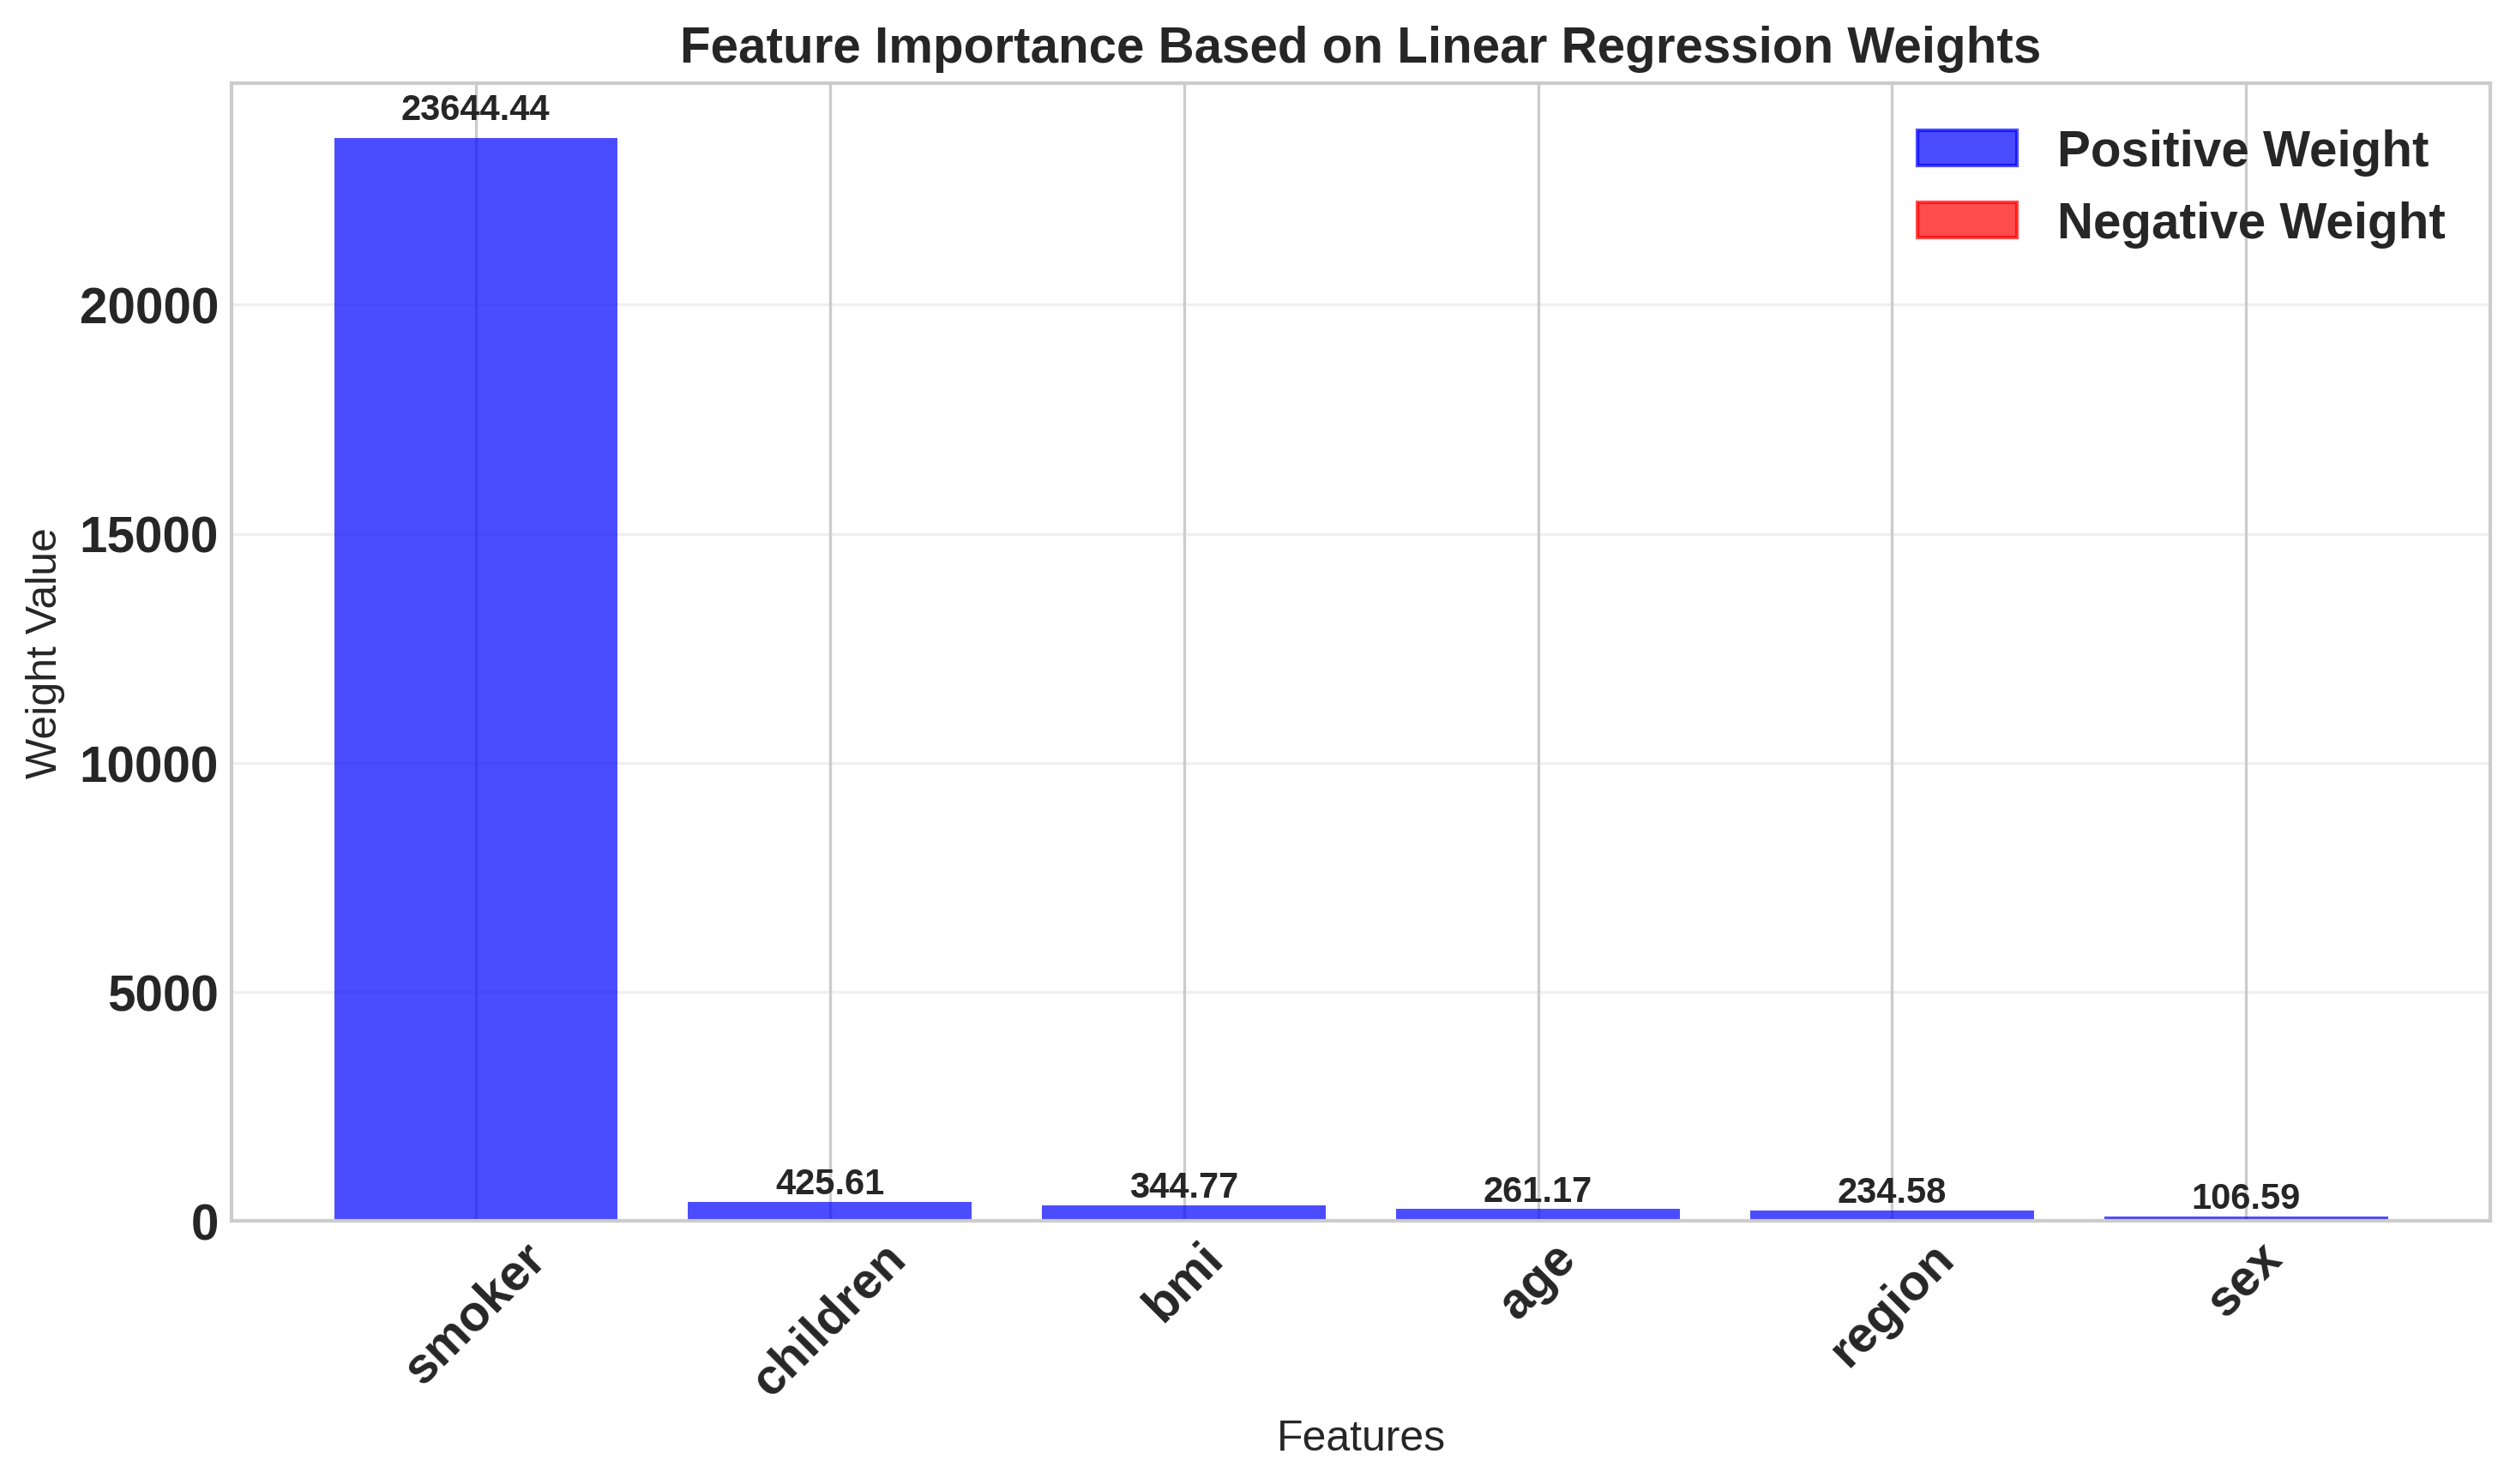
\includegraphics[width=0.8\textwidth]{feature_importance_weights.png}
\caption{Visual representation of feature importance based on linear regression weights}
\label{fig:feature_importance_weights}
\end{figure}

\textbf{Key Findings}:
\begin{itemize}
    \item \textbf{Smoking Status}: By far the most influential factor, with smokers paying approximately \$23,644 more than non-smokers, all else being equal.
    \item \textbf{Number of Children}: Each additional child increases insurance charges by approximately \$426.
    \item \textbf{BMI}: Each unit increase in BMI results in approximately \$345 increase in charges.
    \item \textbf{Age}: Each additional year of age increases charges by approximately \$261.
    \item \textbf{Region and Sex}: Relatively minor effects on insurance charges.
\end{itemize}

\newpage
\subsection{Ridge Regression Results}

The Ridge regression analysis demonstrated how regularization affects coefficient estimates:

\begin{figure}[H]
\centering
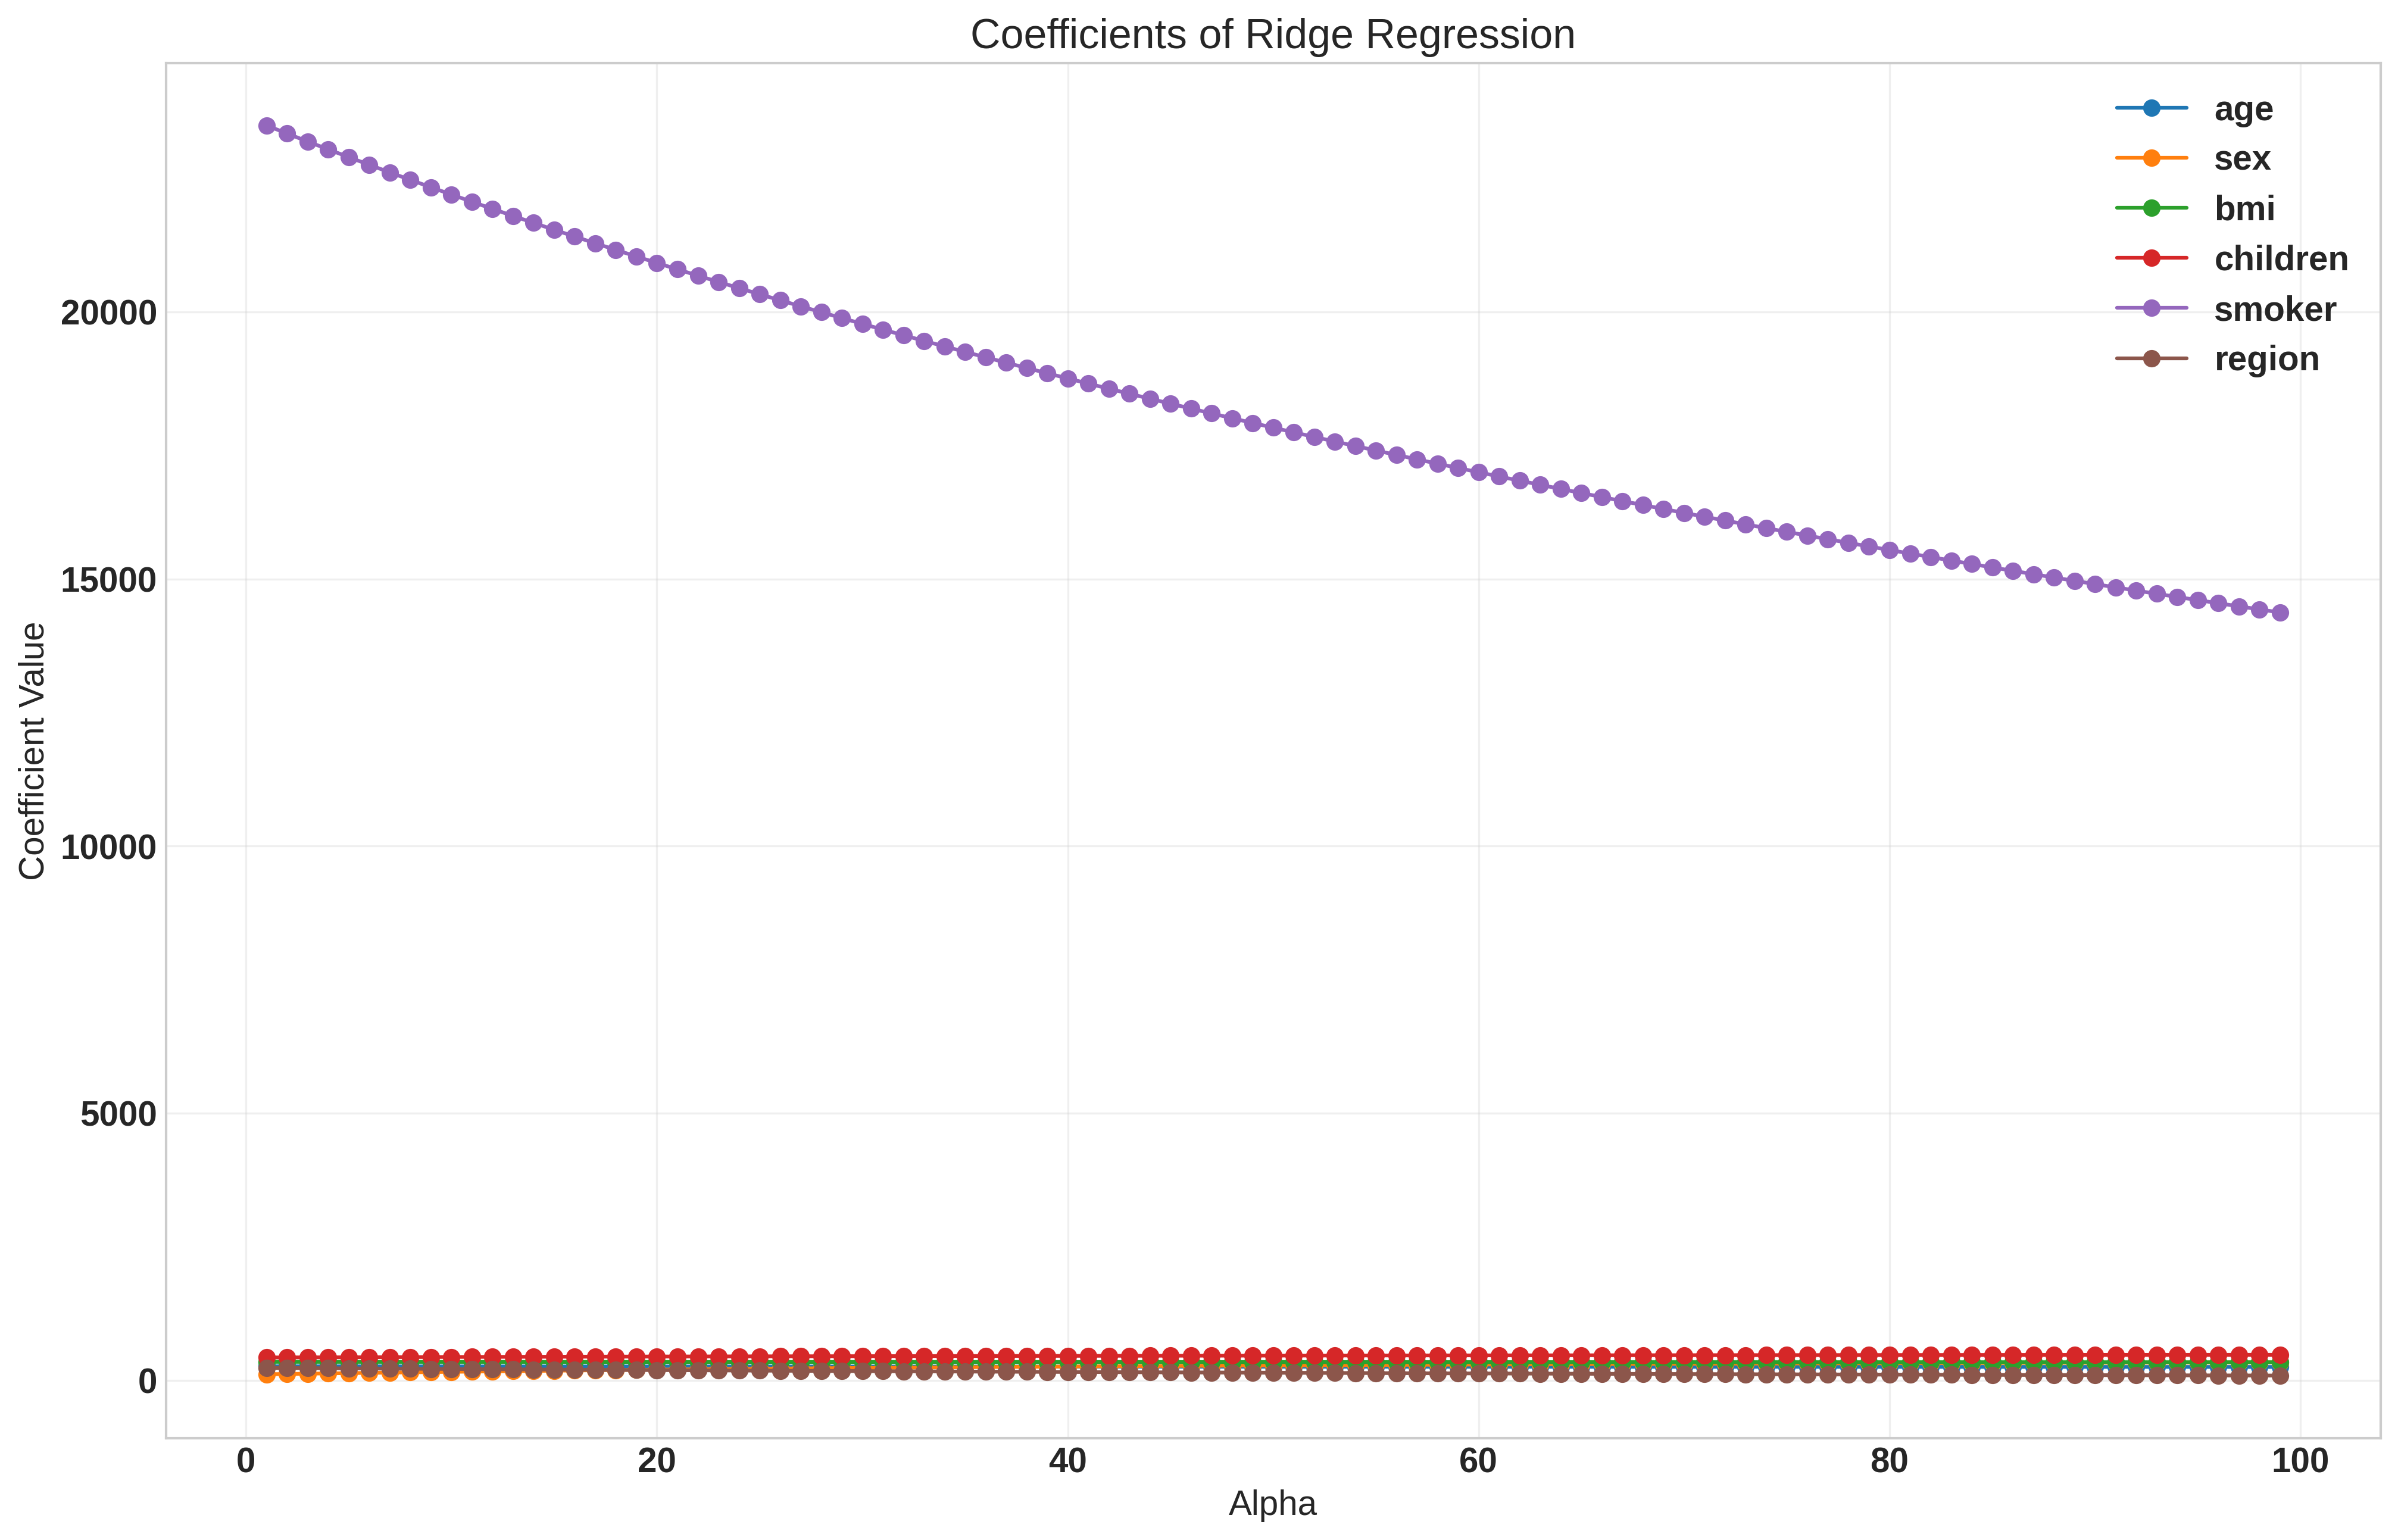
\includegraphics[width=0.9\textwidth]{ridge_regression_coefficients.png}
\caption{Ridge regression coefficients across different alpha values showing regularization paths}
\label{fig:ridge_regression_coefficients}
\end{figure}

\begin{itemize}
    \item At $\alpha = 99$: Smoker coefficient reduced to 14,374.39, showing the regularization effect
    \item Other coefficients showed proportional shrinkage while maintaining relative rankings
    \item The regularization path plots revealed stable coefficient patterns across different $\alpha$ values
\end{itemize}

\subsection{Model Diagnostics Results}

\subsubsection{Linearity and Residual Analysis}
The model diagnostics confirm several important assumptions about the linear regression model:

\begin{figure}[H]
\centering
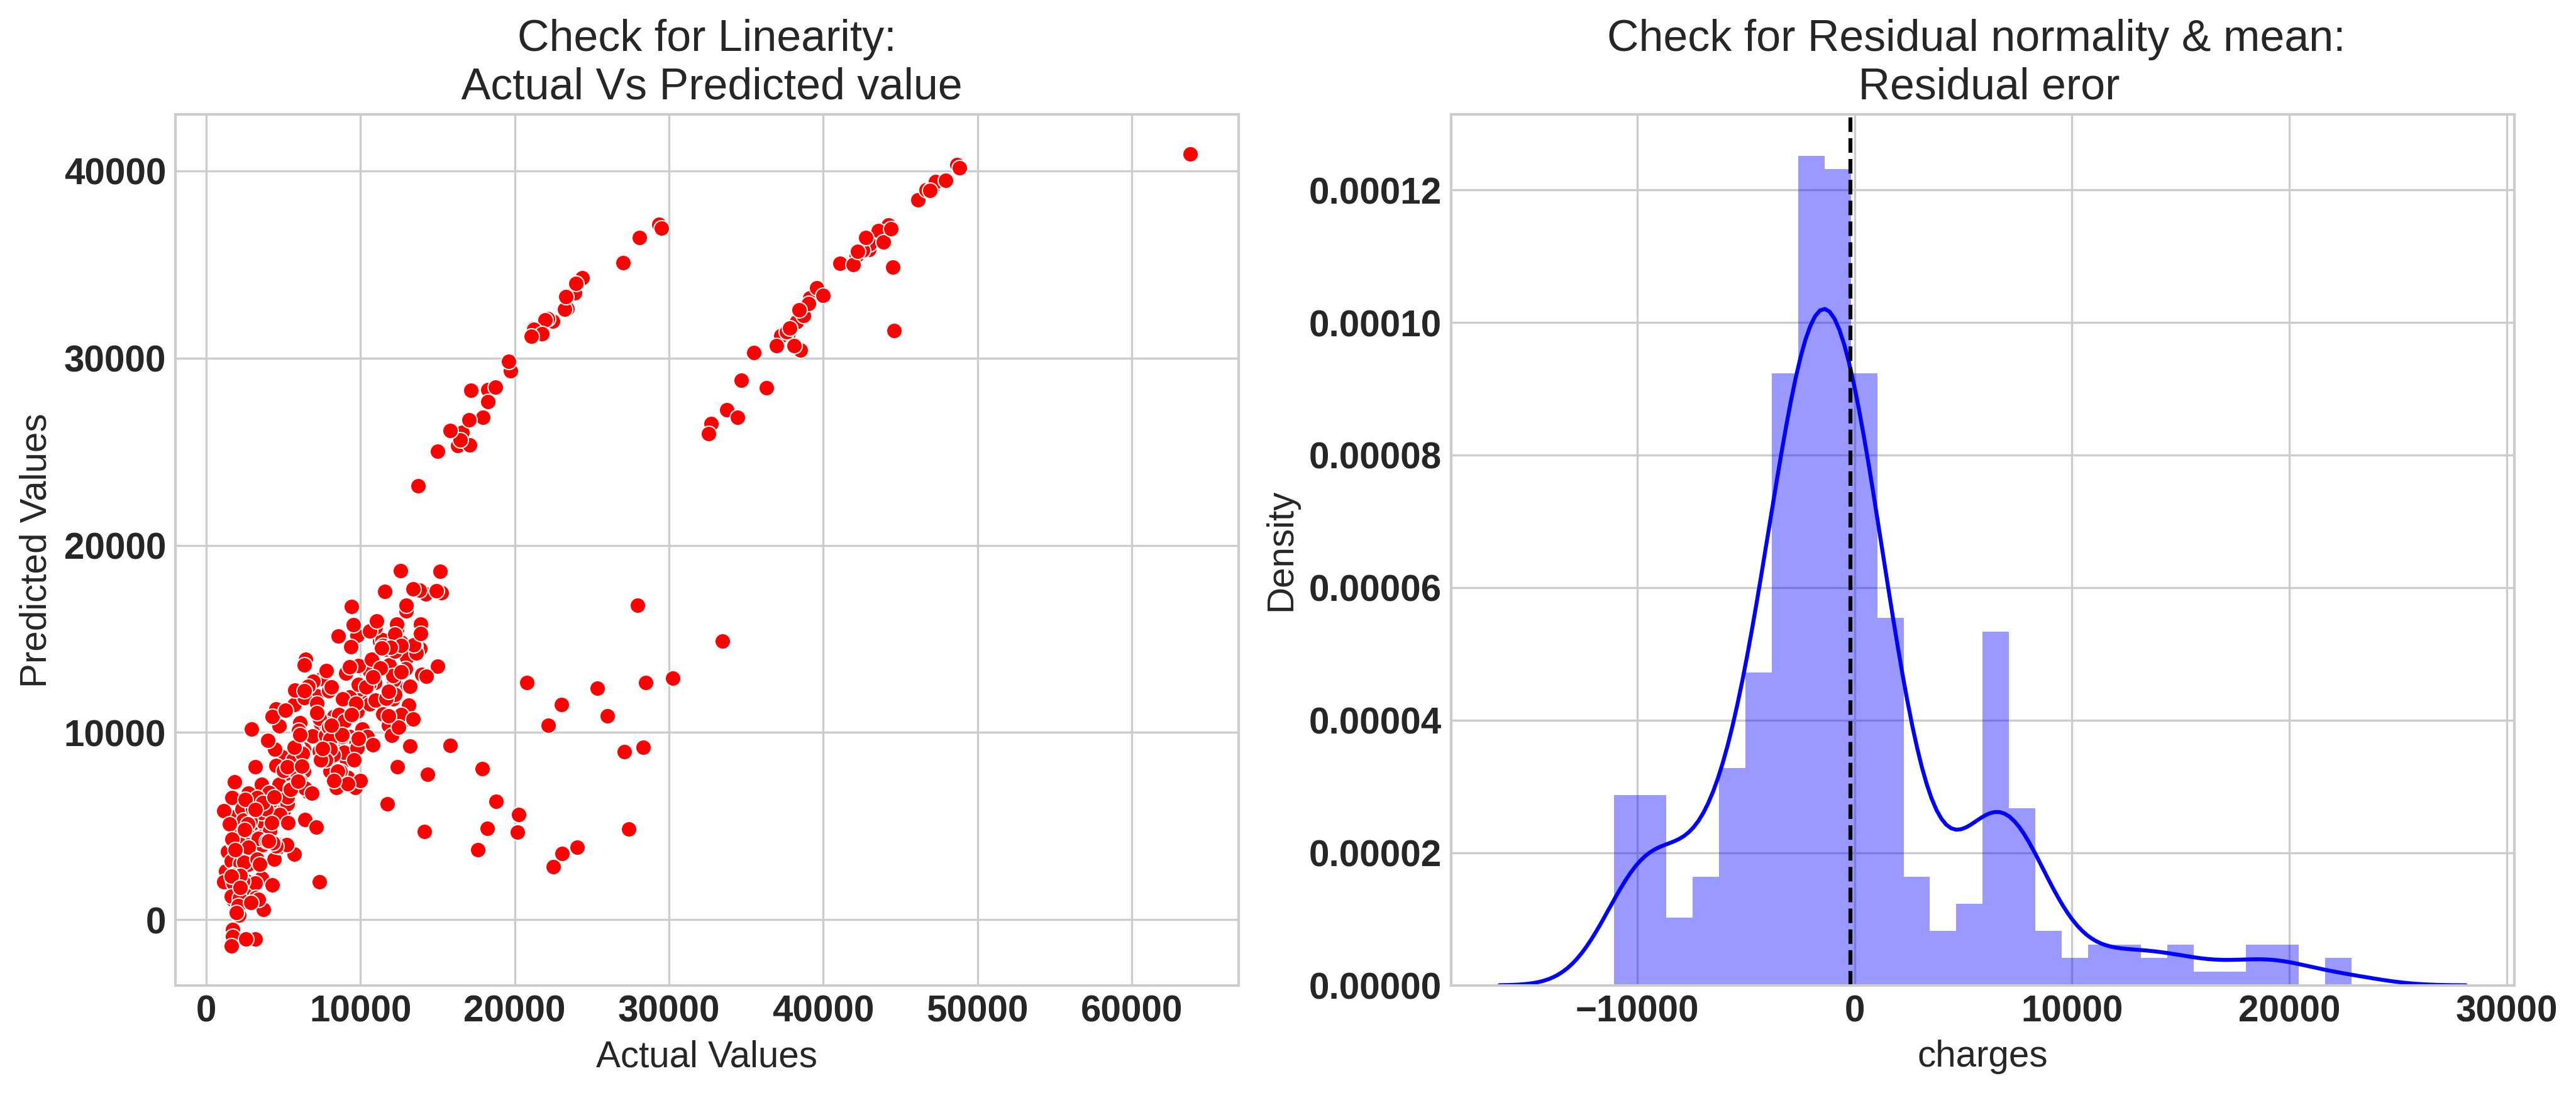
\includegraphics[width=0.9\textwidth]{linearity_check_plots.png}
\caption{Model diagnostics: actual vs predicted values (left) and residual distribution (right)}
\label{fig:linearity_check_plots}
\end{figure}

\textbf{Linearity Check}: The actual vs. predicted values plot demonstrates a strong linear relationship, confirming the appropriateness of linear modeling for this dataset. The points cluster closely around the diagonal line, indicating that the model successfully captures the underlying linear relationships between predictors and the target variable.

\textbf{Residual Analysis}: The residual distribution shows approximately normal distribution with mean near zero, satisfying key model assumptions. The symmetric distribution of residuals around zero indicates that the model is unbiased and that the linear assumptions are appropriate for this data.

\begin{figure}[H]
\centering
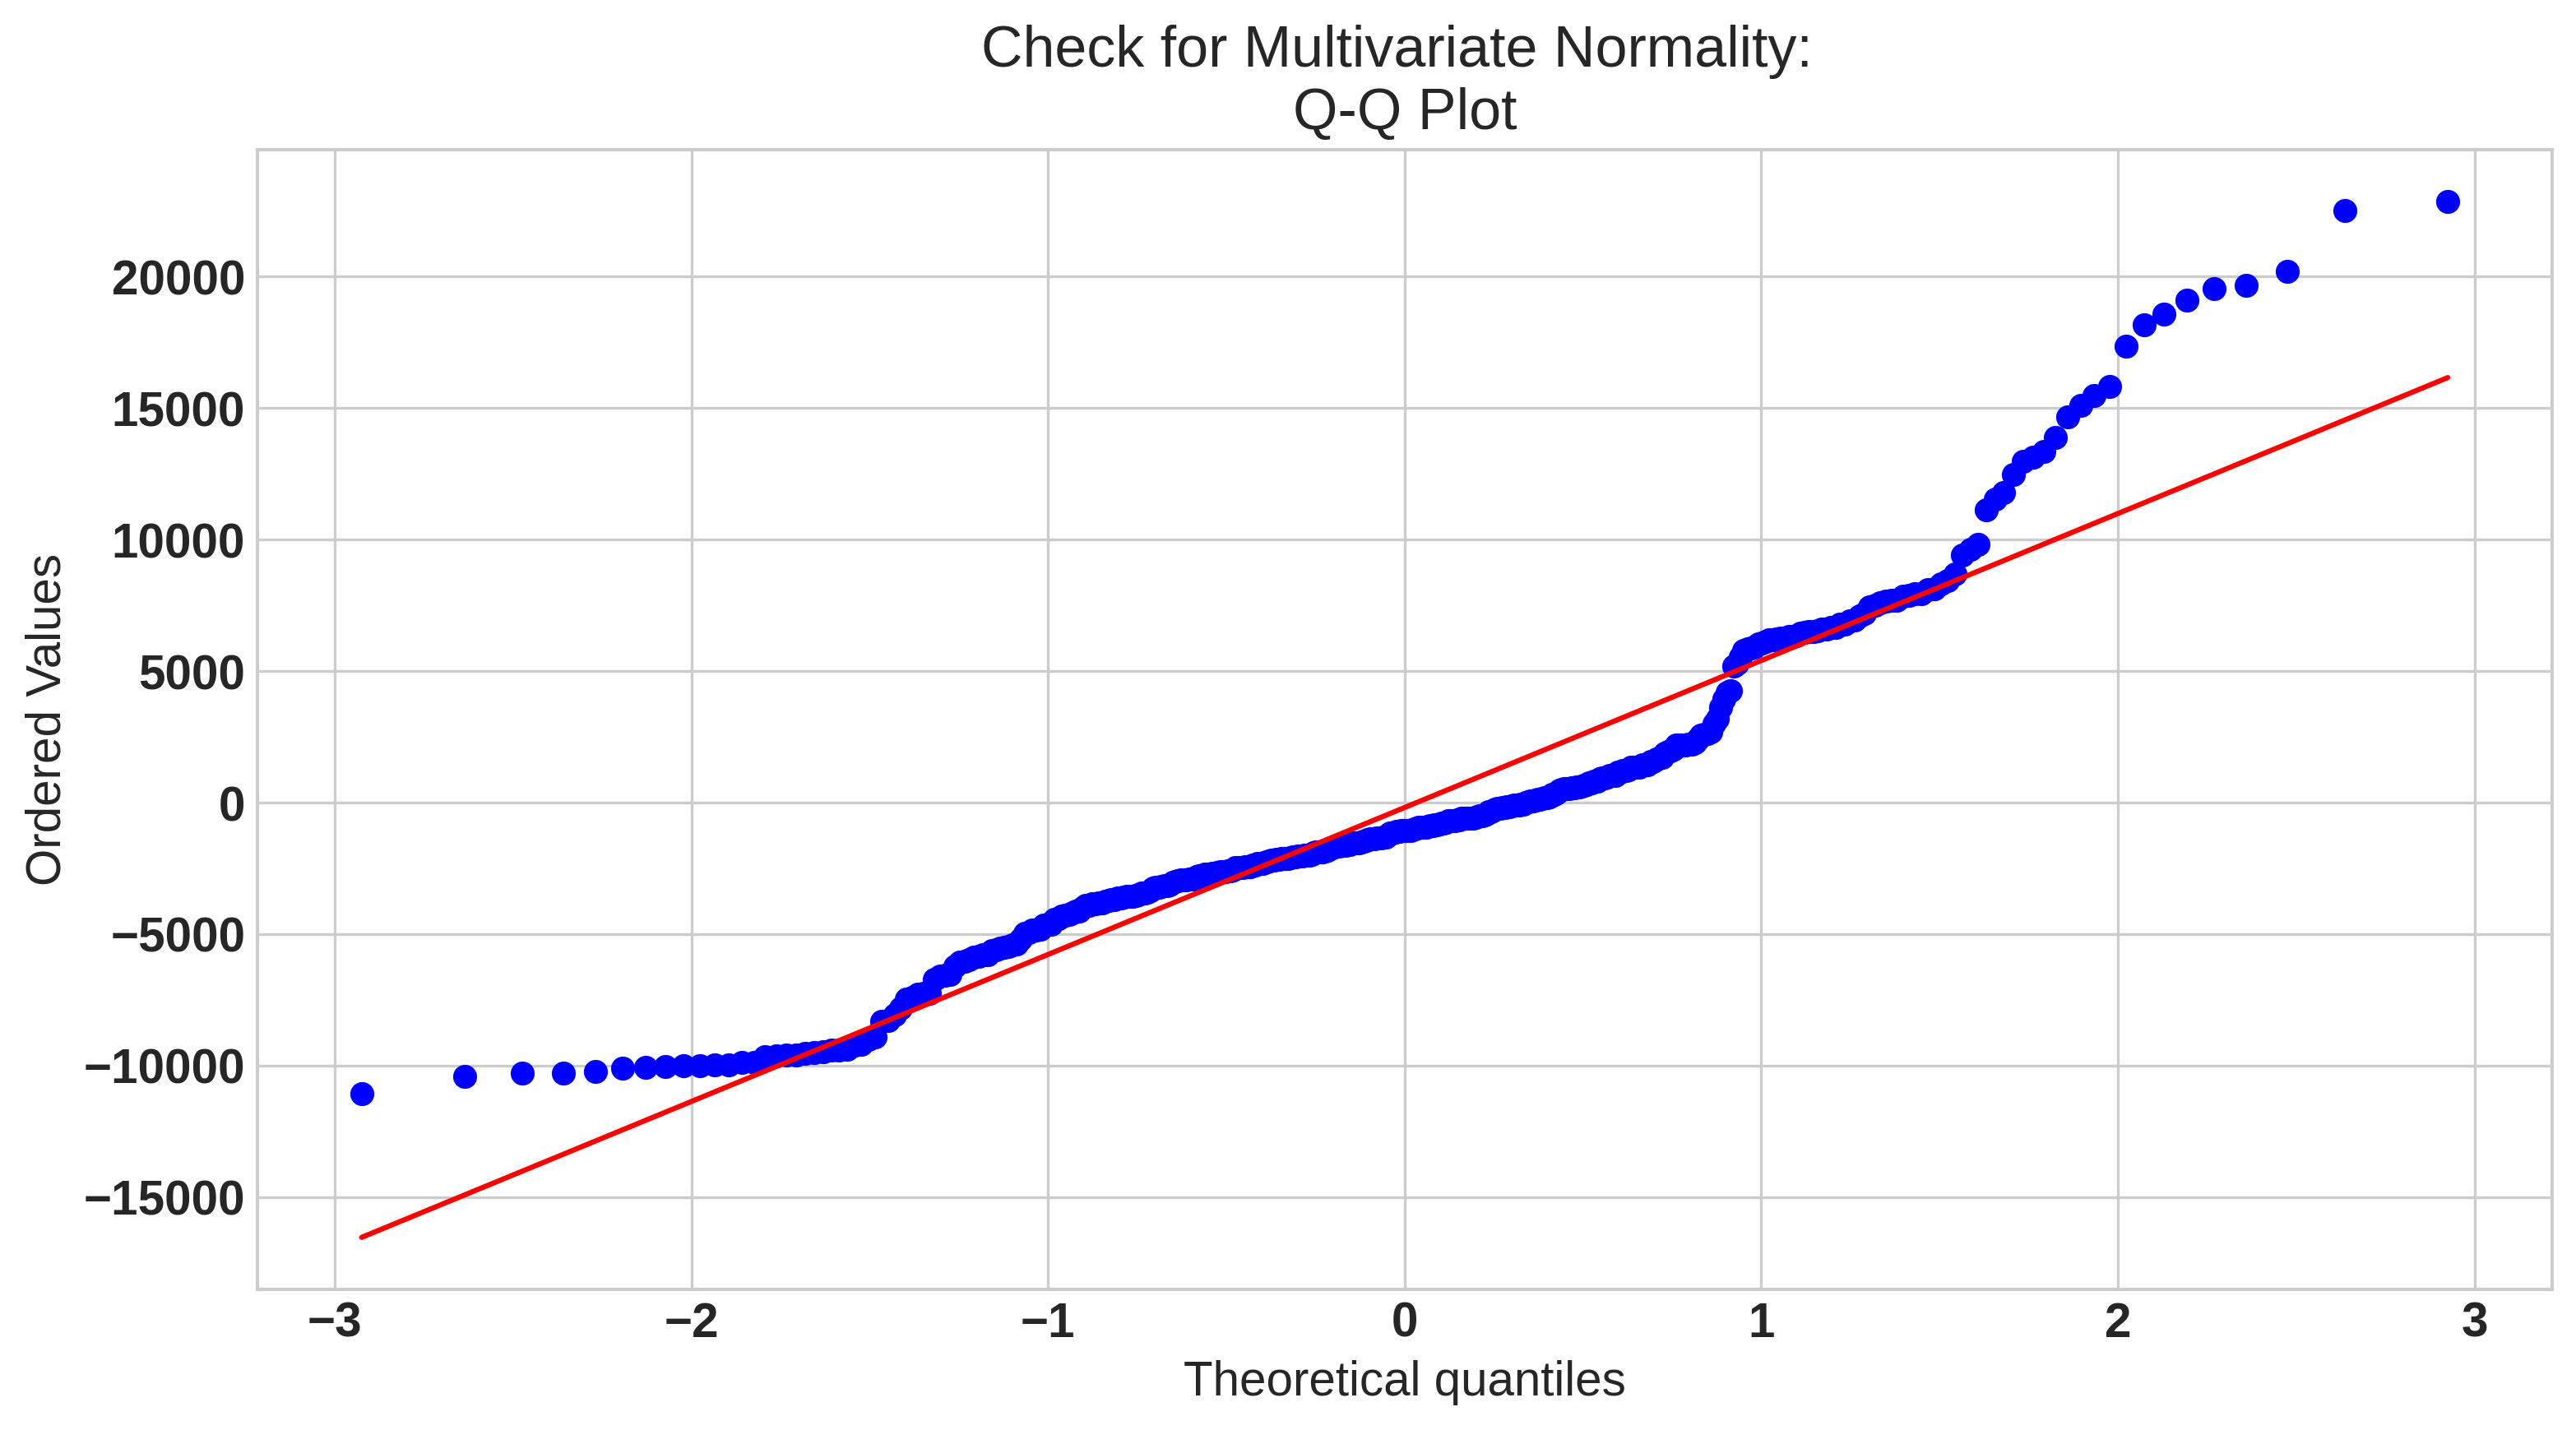
\includegraphics[width=0.9\textwidth]{qq_plot_check.png}
\caption{Q-Q plot for normality check of residuals}
\label{fig:qq_plot_homoscedasticity_check}
\end{figure}

The Q-Q plot further confirms the normality of residuals, with points following closely along the theoretical normal line. This validates the assumption that errors are normally distributed, supporting the reliability of confidence intervals and hypothesis tests for the model coefficients.

\subsubsection{Interaction Effects}

The analysis revealed important interaction effects, particularly:

\begin{figure}[H]
\centering
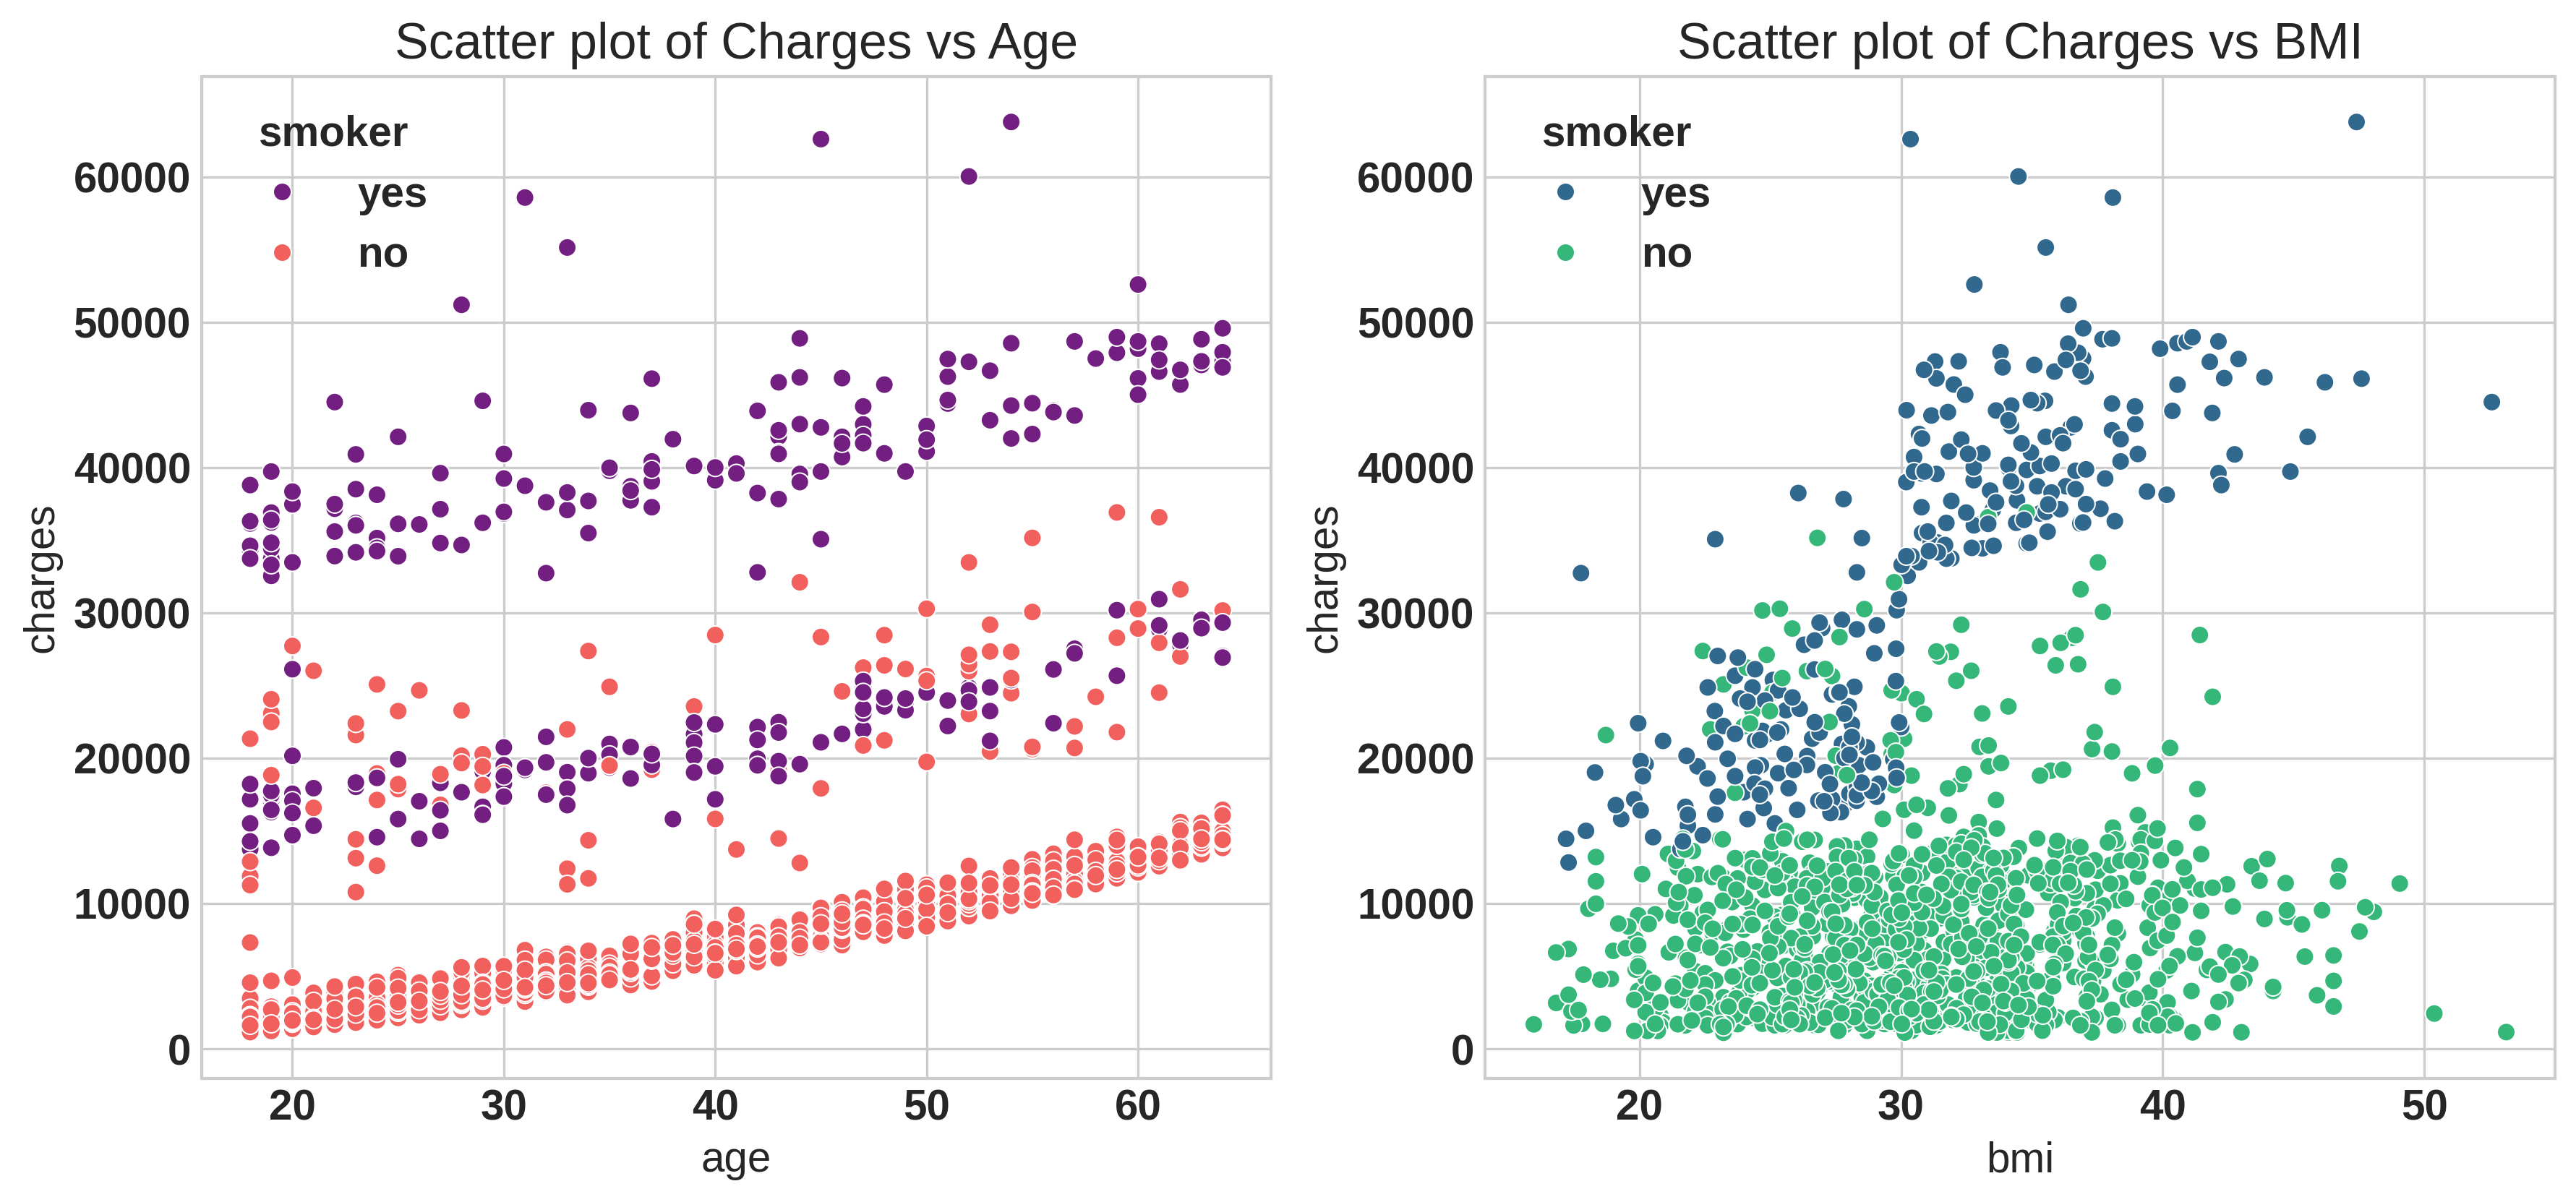
\includegraphics[width=0.9\textwidth]{scatter_plots_charges_vs_age_bmi.png}
\caption{Scatter plots showing interactions between age/BMI and smoking status on charges}
\label{fig:scatter_plots_charges_vs_age_bmi}
\end{figure}

\begin{itemize}
    \item \textbf{BMI × Smoking}: The impact of BMI on charges is significantly amplified for smokers
    \item \textbf{Age × Smoking}: Three distinct charge levels were identified based on age and smoking status combinations
\end{itemize}

These findings suggest that the simple additive model may not fully capture the complexity of insurance charge determination.

\section{Code and Data Availability}

The complete source code, data analysis scripts, and datasets used in this study are available in the GitHub repository: \url{https://github.com/pleyva2004/Statistical-Learning-Capstone}. The repository includes Jupyter notebooks for data analysis, visualization scripts, and all generated figures referenced in this report.

\section{Conclusion}

This comprehensive statistical analysis of insurance charges has yielded several important conclusions:

\subsection{Primary Findings}

\subsubsection{Smoking Status Dominance}
The analysis unequivocally demonstrates that smoking status is the most critical factor in determining insurance charges, with an effect magnitude far exceeding all other variables combined. This finding aligns with medical evidence regarding smoking-related health risks and associated healthcare costs.

\subsubsection{Model Performance}
The linear regression model achieved satisfactory performance with an R-squared of 0.769, indicating that the selected demographic and health-related variables explain approximately 77\% of the variance in insurance charges. This level of explanatory power suggests that the model captures the major determinants of insurance pricing.

\subsubsection{Feature Hierarchy}
A clear hierarchy of feature importance emerged: smoking status >> children > BMI > age > region $\approx$ sex. This ranking provides valuable insights for both insurance companies and policyholders regarding factors that most significantly impact premiums.

\subsection{Methodological Insights}

\subsubsection{Linear Model Adequacy}
    Despite the complexity of insurance pricing, linear regression proved effective for this dataset, though the presence of interaction effects suggests that more sophisticated models might capture additional variance.

\subsubsection{Regularization Effects}
    Ridge regression demonstrated how regularization can provide more stable coefficient estimates, particularly valuable when deploying models in production environments where robustness is crucial.

\subsection{Practical Implications}

\textbf{For Insurance Companies}:
\begin{itemize}
    \item Smoking status should be weighted heavily in risk assessment models
    \item The identified feature importance hierarchy can inform pricing strategy development
    \item The model provides a foundation for actuarial analysis and rate setting
\end{itemize}

\textbf{For Policyholders}:
\begin{itemize}
    \item Smoking cessation represents the single most impactful action for reducing insurance premiums
    \item BMI management can provide meaningful cost savings
    \item Demographic factors (sex, region) have minimal impact on charges
\end{itemize}

\subsection{Limitations and Future Research}

\textbf{Model Limitations}:
\begin{itemize}
    \item Interaction effects are not fully captured in the simple additive model
    \item The dataset may not include all relevant predictors (e.g., pre-existing conditions, lifestyle factors)
\end{itemize}

\textbf{Future Research Directions}:
\begin{itemize}
    \item Investigation of non-linear models and interaction terms
    \item Incorporation of additional health and lifestyle variables
    \item Time-series analysis to understand temporal trends in insurance pricing
    \item Advanced machine learning approaches for improved prediction accuracy
\end{itemize}

\subsection{Final Remarks}

This study successfully demonstrates the application of statistical learning techniques to understand insurance charge determination. The findings provide actionable insights for stakeholders in the insurance industry while highlighting the paramount importance of smoking status in healthcare cost prediction. The developed models serve as a foundation for more sophisticated insurance pricing systems and provide a framework for future research in this domain.

The results underscore the critical role of lifestyle factors, particularly smoking, in healthcare costs and insurance pricing, reinforcing the importance of public health initiatives aimed at smoking prevention and cessation. From a statistical modeling perspective, this study illustrates the effectiveness of linear regression for interpretable insurance pricing models while identifying areas for methodological enhancement in future research.

\end{document}
